% =====================================================================
% Full-length paper (IEEE Transactions style, no page limit).
% Every number is read from tm_ris_ofdm/results/*.json; Appendix D maps each
% table and figure to the script that produced it. Derived numbers (coherence
% times, unknown counts, operation counts, energy fractions) are computed in the
% text or in Appendix C. \TODO marks items that still need checking.
% =====================================================================
\documentclass[journal,onecolumn,11pt,draftclsnofoot]{IEEEtran}
\usepackage{amsmath,amssymb,amsthm,bm,graphicx,booktabs,cite,multirow,array}
\usepackage{algorithm,algpseudocode}
\usepackage{xcolor}
\usepackage[hidelinks]{hyperref}
\newcommand{\TODO}[1]{\textcolor{red}{[TODO: #1]}}
\DeclareMathOperator{\diag}{diag}
\DeclareMathOperator{\vect}{vec}
\DeclareMathOperator{\tr}{tr}
\newtheorem{proposition}{Proposition}
\newtheorem{corollary}{Corollary}
\theoremstyle{remark}\newtheorem{remark}{Remark}
\graphicspath{{../../figures/}}
\renewcommand{\arraystretch}{1.15}

\begin{document}
\title{A Timing-Only Receiver for OFDM through\\ Dispersive Time-Modulated Reconfigurable Intelligent Surfaces}
\author{\TODO{authors and affiliations}}
\maketitle

\begin{abstract}
A time-modulated reconfigurable intelligent surface (TM-RIS) switches its elements
several times within each OFDM symbol. The switching creates harmonics that couple
every received subcarrier to many transmitted ones, and when the elements are
frequency dispersive, as real varactor cells are, the coupling matrix is neither
diagonal nor Toeplitz. Existing TM-RIS systems therefore treat the coupling as
interference, which caps the rate of the legitimate receiver at the
signal-to-harmonic-interference ratio, and a recent physically consistent model of
the dispersive TM-RIS channel leaves receiver design open. This paper builds that
receiver around one structural fact: grouping the harmonic expansion by switching
state separates the coupling into Toeplitz factors fixed by the switching timing,
which the receiver knows, and per-state input responses that absorb both the
propagation and the element dispersion, which it does not. Every receiver block
follows from this separation: a pilot-based low-rank estimator that needs no
element model; a blind estimator of the RIS clock offset and of the delay reference, based on the
observation that an offset is exactly an opposite delay of the two hops, which makes a
wrong offset overfit the pilots; a two-timescale extension
that learns the static base-station--RIS side once; warm-started updates; and an
exact matrix-free equalizer. In an extensive evaluation with the published cell of
the anchor model, physical and 3GPP channels, mobility, hardware impairments and
coding, the receiver is within 0.1\,bit/s/Hz of perfect channel knowledge with two
pilot symbols on a shared-path channel and within 0.2 with four to eight on 3GPP TDL-C at 20\,dB; in a
pre-registered comparison in which every baseline gets a robust equalizer, it beats the best baseline on every
channel by 0.3--0.4\,bit/s/Hz at 20\,dB and 1.1--2.2 at 30\,dB, and with two pilot symbols exceeds a full-harmonic
basis-expansion estimator given 32,
decodes coded blocks within 0.14\,dB of perfect knowledge where the conventional receiver never decodes, absorbs an
unknown clock offset blindly with no rate loss against known timing, and keeps 3.9--5.7\,bit/s/Hz net of pilot overhead on 3GPP TDL channels from
walking speed to 120\,km/h. All limits found, including failed attempts, are reported.
\end{abstract}

\begin{IEEEkeywords}
Reconfigurable intelligent surface, time modulation, space-time coding, OFDM,
intercarrier interference, channel estimation, synchronization, equalization.
\end{IEEEkeywords}

\section{Introduction}\label{sec:intro}

\subsection{Context and problem}
A reconfigurable intelligent surface (RIS) shapes the radio channel with many
passive, electronically switched elements~\cite{basar2019,wu2019}. Most RIS work
keeps the configuration fixed during an OFDM symbol and changes it, if at all,
between symbols. A \emph{time-modulated} RIS (TM-RIS), also called a
space-time-coding metasurface, instead switches each element several times within
the symbol~\cite{zhang2018}. The reflected signal then contains harmonics of the
switching frequency, and the surface can steer, scramble or split energy across
frequency as well as space. OFDM-aligned time modulation has been proposed for
waveform security and directional modulation~\cite{xu2023tmirs,tao2025gflownet,wang2026generative}
and for joint sensing and security~\cite{tao2025isac}.

For the user that the surface serves, the same harmonics are a problem. A harmonic
at $h$ times the subcarrier spacing moves energy from transmitted subcarrier $m$ to
received subcarrier $m+h$, so the frequency-domain channel matrix is no longer
diagonal. Iudice \emph{et al.}~\cite{iudice2026} recently derived a physically
consistent model of this channel in which each element has a frequency-dispersive
(finite-memory) response, as a real varactor cell does. They showed that a
generalized cyclic prefix removes inter-symbol interference but that the coupling
between subcarriers remains for any prefix length, and that with dispersive elements
the coupling matrix is not even Toeplitz. Receiver design was explicitly left open.

How large is the problem? For a two-state element with ideal reflection $\pm1$ and
duty cycle $D$ (fraction of the period in state 1), Parseval's theorem gives the
fraction of reflected energy that stays on the original subcarrier as
$(2D-1)^2$ (Appendix~\ref{app:parseval}). At $D=0.75$ only 25\% stays; the
remaining 75\% is spread over the other harmonics. A conventional one-tap OFDM
receiver treats that 75\% as interference, so its signal-to-interference ratio is
at most $(2D-1)^2/(1-(2D-1)^2)=-4.8$\,dB, and its rate saturates however high the
SNR. In our evaluation the one-tap receiver delivers 0.42\,bit/s/Hz at both 20 and
30\,dB, against 6.6 and 9.9\,bit/s/Hz with perfect channel knowledge and joint
equalization (Section~\ref{sec:res-est}).

Time modulation does not, by itself, give the user more rate: for a single user, an optimized \emph{static} RIS
delivers more (Section~\ref{sec:res-motiv}). A TM-RIS is deployed for its other functions, such as directional
security, harmonic steering of several users or sensing, and the question this paper answers is how much of the
resulting loss the legitimate receiver can win back. Recovering this rate requires the full coupling matrix at the receiver. The matrix
has up to $M^2$ entries ($M=3276$ subcarriers in a 100\,MHz 5G NR carrier) and
depends on the propagation on both hops, on the switching pattern, and on the
element response. A generic estimator of a non-diagonal OFDM channel, such as the
basis-expansion model used for high-mobility channels~\cite{tang2007}, does not
know where the coupling comes from. It must estimate every harmonic separately.
Because rectangular switching leaves a slowly decaying $1/h^2$ energy tail, it
either truncates (and then misses 3.4\% of the energy at $|h|\le 12$, which caps its
accuracy near $-15$\,dB) or keeps all harmonics (and then needs many pilots).

\subsection{Central idea}
The receiver of a TM-RIS link is in an unusual position: it knows \emph{how} the
channel varies inside the symbol, because the variation is the switching pattern,
and the switching pattern is set by the network. What it does not know is the
propagation and the exact element response. This paper turns that observation
into an exact structural statement and builds the entire receiver on it.

Grouping the harmonic expansion of~\cite{iudice2026} by element \emph{state} rather
than by harmonic gives (Proposition~\ref{prop:sep})
\begin{equation*}
\bm H=\sum_{q=1}^{Q}\sum_{s=1}^{2}\underbrace{\bm T_{q,s}}_{\text{timing only}}\circ
\big(\underbrace{\bm a^{\rm d}_q}_{\text{user hop}}\,
(\underbrace{\bm\Gamma_s\odot\bm a^{\rm s}_q}_{\text{BS hop and dispersion}})^{\!\top}\big),
\end{equation*}
where each $\bm T_{q,s}$ is a Toeplitz matrix fixed by the switching timing alone.
The algebra is a regrouping of~\cite[eq.~(5)]{iudice2026}, and we credit it as such.
What is new is what the regrouping implies for a receiver. Each consequence becomes
one block of the receiver:
\begin{enumerate}
\item The element dispersion multiplies only the input side, together with the
unknown base-station (BS)--RIS channel, so it can be absorbed into an unknown
per-state input response. \emph{The receiver needs no element model}
(Section~\ref{sec:est}). Assuming the ideal $\pm1$ element of earlier work costs
1.4/6.6\,dB at 20/30\,dB; the timing-only receiver loses 0.08/0.11\,dB.
\item All elements see the same propagation paths, so the unknown factors live in a
low-dimensional delay subspace shared by all elements and both states. The unknowns
fall from up to $M^2$ to about $3Lr$ ($L$ delay functions, rank $r$), and two pilot
symbols suffice for a sparse channel (four to eight for 3GPP TDL-C at 100\,ns).
\item A clock offset between the RIS and the receiver changes $\bm T_{q,s}$ to
$\bm D\bm T_{q,s}\bm D^{*}$, which is \emph{exactly} a delay of the user hop and an
advance of the BS hop. This explains why a pilot-residual timing search fails at high
SNR (the delays absorb the offset), and why the Bayesian evidence, which also asks how
probable the absorbing delays are, recovers it (Section~\ref{sec:timing}).
\item The BS--RIS side does not move, so it can be learned once over many frames, and
each new frame estimates only the user side (Section~\ref{sec:twoscale}).
\item Each $\bm T_{q,s}\bm x$ is a linear convolution, so products with $\bm H$ cost
$\mathcal O(QM\log M)$ and the MMSE equalizer can run matrix-free
(Section~\ref{sec:eq}).
\item The $1/h$ amplitude envelope of $\bm T_{q,s}$ explains, quantitatively, why
truncated estimators and banded equalizers fail on this channel
(Corollary~\ref{cor:tail}).
\end{enumerate}

\subsection{Contributions}
\begin{itemize}
\item \textbf{C1, receiver structure.} To our knowledge, the first pilot-based receiver for OFDM through a
(dispersive) TM-RIS: pilot-based estimation of the complete coupling matrix and joint
equalization, organized around the timing/propagation separation above
(Fig.~\ref{fig:pipeline}, Algorithms~\ref{alg:est}--\ref{alg:cg}).
\item \textbf{C2, timing-only estimation.} Absorbing the dispersion into the unknown
input response, so that no element model, calibration or resonance knowledge is needed,
and a low-rank shared-subspace estimator that covers identical, cyclically shifted and
arbitrary per-element switching patterns in one form.
\item \textbf{C3, blind clock-offset recovery.} The opposite-delay identity for a
TM-RIS clock offset and its physical meaning (bulk hop delays cancel if the RIS follows the incident signal;
the BS--RIS delay becomes an offset if it follows the BS clock), the resulting overfitting mechanism of
residual-based timing, and an evidence-based estimator of the offset and the delay reference that absorbs the offset from two pilot symbols
with no rate loss against known timing. (Because of the identity, the offset is defined only
relative to the reference of the delay prior; the meaningful metric is the rate loss.)
\item \textbf{C4, exhaustive evaluation.} An evaluation against the strongest
baselines we could build (full-harmonic basis expansion given 16$\times$ more pilots,
sparse recovery, unstructured least squares, literature equalizers given the true
channel), on physical and 3GPP channels, with coding, mobility and pilot overhead,
hardware impairments, timing errors, multiple panels and interference, and the
complexity in operations and measured time. Pass/fail criteria were fixed before each
experiment; failures are reported with their diagnosis.
\end{itemize}

We adopt, and do not claim: low-rank modelling of RIS cascaded
channels~\cite{wang2020compressed}; the DPSS delay basis~\cite{slepian1978,zemen2005};
matrix-free iterative equalization through product-convolution
operators~\cite{hrycak2010} (here the representation is exact rather than a
basis-expansion approximation); learning the quasi-static BS--RIS channel on a slow
timescale~\cite{hu2019twotimescale}; Bayesian evidence for model and timing
selection~\cite{mackay1992,access2019bayes}; and the observation, known from
space-time-coding metasurfaces, that a time shift of the switching pattern multiplies
harmonic $h$ by a linear phase~\cite{zhang2018}. Section~\ref{sec:related} explains
how each differs from its use here.

\subsection{Organization and notation}
Section~\ref{sec:related} positions the work. Section~\ref{sec:model} gives the system
model and every assumption with its justification. Section~\ref{sec:structure} derives
the structure of the coupling. Section~\ref{sec:receiver} presents the receiver,
algorithm by algorithm, with its complexity. Section~\ref{sec:method} describes the
evaluation protocol and baselines, Section~\ref{sec:results} the results, and
Section~\ref{sec:tradeoffs} the trade-offs and limitations.

Bold lower- and upper-case letters denote vectors and matrices; $\circ$ and $\odot$ are
the Hadamard product of matrices and vectors; $(\cdot)^{\top}$, $(\cdot)^{\mathsf H}$ and
$(\cdot)^{*}$ are transpose, conjugate transpose and conjugate; $\diag(\bm a)$ is the
diagonal matrix with $\bm a$ on its diagonal; $\vect(\cdot)$ stacks columns;
$\mathcal{CN}(\bm\mu,\bm C)$ is the circularly symmetric complex Gaussian distribution;
$\mathrm{sinc}(x)=\sin(\pi x)/(\pi x)$. Confidence intervals are $\pm1.96\,s/\sqrt{n}$
over $n$ independent channel draws.

\section{Related Work and Positioning}\label{sec:related}

\subsection{Time-modulated surfaces and OFDM}
Space-time-coding digital metasurfaces~\cite{zhang2018} control harmonics by the
switching pattern: a time delay of an element's pattern multiplies harmonic $h$ by a
linear phase, which steers harmonic beams. In communications, time-modulated
intelligent reflecting surfaces aligned with OFDM symbols have been designed for
waveform security, so that the intended direction receives an undistorted signal and
other directions receive scrambled symbols~\cite{xu2023tmirs}; pattern design has been
cast as generative search~\cite{tao2025gflownet,wang2026generative} and extended to
sensing~\cite{tao2025isac}. In this line of work the legitimate receiver is a
conventional OFDM receiver and the harmonic coupling it sees is either designed to be
small in its direction or treated as interference. All of it uses an ideal,
frequency-flat element. The only work that undoes the mixing is an attack: an
eavesdropper recovers directional-modulation symbols by blind independent component
analysis, resolving ambiguities with the Toeplitz structure that the ideal model
implies~\cite{tao2025secure}. Rapidly time-varying RIS have also been analysed without
OFDM~\cite{verde2023}. Iudice \emph{et al.}~\cite{iudice2026} gave the first physically
consistent model with dispersive elements, showed that dispersion breaks the Toeplitz
structure, and listed equalization across coupled subcarriers as open.

Closest in spirit outside RIS are OFDM backscatter systems, in which a tag switches its reflection within OFDM
symbols: the receiver there decodes the \emph{tag's} data from the switching, or avoids the resulting intercarrier
interference with unused subcarriers~\cite{liu2021tscatter,bsici2024,sr2024free}; space-time-coding metasurfaces
have also been used for sensing from harmonic amplitudes and for non-coherent modulation~\cite{stcisac2025,stcdiff2025}.
Linear periodically time-varying channels are well studied in power-line communication, but with periods much
longer than a symbol and hence no harmonic coupling at the subcarrier spacing~\cite{plc_lptv}.

\emph{Difference.} We design the legitimate receiver for the dispersive model: we
estimate and equalize the coupling instead of treating it as interference, and our
estimator does not rely on a Toeplitz (ideal-element) structure, which dispersion breaks.

\subsection{Estimating non-diagonal OFDM channels}
Intra-symbol channel variation from Doppler makes the OFDM channel matrix
non-diagonal. The standard estimator expands the time variation on a basis: complex
exponentials (CE-BEM)~\cite{tang2007}, or discrete prolate spheroidal
sequences~\cite{zemen2005}, giving a banded frequency-domain matrix with one unknown
gain profile per harmonic. Sparse recovery over harmonic--delay dictionaries
(orthogonal matching pursuit~\cite{tropp2007}) is an alternative. These methods assume
that the time variation is \emph{unknown}; they must estimate it.

\emph{Difference.} For a TM-RIS the time variation is known, up to the propagation
and the element response. Our estimator uses the known timing and estimates only the
static propagation (with the dispersion absorbed). The difference is large in
practice: with two pilot symbols CE-BEM reaches 2.2/1.1\,bit/s/Hz at 20/30\,dB against
our 6.5/9.7, and a full-harmonic CE-BEM needs 32 pilot symbols to approach our
two-pilot result (Section~\ref{sec:res-est}). We use CE-BEM, with the same delay prior
as ours, as the main baseline.

\subsection{Equalization of non-diagonal OFDM channels}
Banded MMSE equalizers keep only the strongest neighbouring subcarriers~\cite{schniter2004,rugini2005}.
Iterative Krylov solvers (LSQR, GMRES) with fast products through product-convolution
operators equalize a basis-expansion channel without forming the matrix~\cite{hrycak2010}.

\emph{Difference.} We adopt the iterative approach. For a TM-RIS the product-convolution
form is exact (Proposition~\ref{prop:sep}), not a basis-expansion approximation, and for
identical patterns all elements share one kernel per state, so a product needs one
batched FFT per state. Banded equalizers fail here even with the true channel, because
of the $1/h$ harmonic envelope (Section~\ref{sec:res-est}).

\subsection{RIS channel estimation}
Conventional RIS channel estimation assumes a configuration that is constant during
each OFDM symbol and changes it between symbols, so that the cascaded channel can be
separated~\cite{zheng2020ofdm}; low-rank and sparse structure of the cascaded channel is
widely exploited~\cite{wang2020compressed}. Two-timescale schemes estimate the
quasi-static BS--RIS channel rarely and the mobile RIS--user channel often~\cite{hu2019twotimescale}.

\emph{Difference.} None of these handles switching inside the symbol, where each
received subcarrier mixes many transmitted ones. We use low-rank structure and the
two-timescale principle, but inside the harmonic-coupled model, where the static side
also carries the element dispersion.

\subsection{Synchronization}
Timing offsets between RIS reflection patterns and the receiver have been studied for
distributed multi-RIS systems with maximum-likelihood estimators~\cite{zhao2022multiris}
and for RIS-assisted symbiotic radio, where the RIS modulates its own data and an
unknown offset causes intercarrier interference that is estimated blindly from virtual
subcarriers~\cite{chen2024sr}. Bayesian model selection and model averaging over timing
offsets have been used in OFDM channel estimation~\cite{access2019bayes,hku2010}, building
on the evidence framework~\cite{mackay1992}.

\emph{Difference.} We show that for a TM-RIS a clock offset is exactly an opposite
delay shift of the two hops. Consequently the pilot residual is nearly flat in the
offset, a fact that explains the failure of residual search at high SNR and motivates
evidence-based estimation. We use the evidence of our own first-stage model; the tool
is known, its necessity and its use here are not.

\begin{table}[!htbp]\centering
\caption{Capabilities of existing approaches and of the proposed receiver for OFDM through a TM-RIS.
``Pilots'' is the number of OFDM pilot symbols needed to come within 0.3\,bit/s/Hz of perfect channel knowledge at 20\,dB in our setting, pre-registered fair rerun with 30 channels and the robust equalizer for every estimator (Table~\ref{tab:fair}); $>32$: not reached with 32.}
\label{tab:features}
\resizebox{\textwidth}{!}{%
\begin{tabular}{p{4.4cm}ccccccc}\toprule
Approach & \parbox{1.3cm}{\centering in-symbol\\ switching} & \parbox{1.2cm}{\centering dispersive\\ element} & \parbox{1.4cm}{\centering element\\ model needed} & \parbox{1.3cm}{\centering full\\ coupling} & pilots & \parbox{1.3cm}{\centering clock\\ offset} & \parbox{1.6cm}{\centering cost per\\ $\bm H\bm x$} \\\midrule
One-tap OFDM (TM-IRS designs~\cite{xu2023tmirs,tao2025gflownet}) & coupling as noise & -- & -- & no & 1 & -- & $M$ \\
Blind ICA attack~\cite{tao2025secure} & yes & no (Toeplitz) & ideal & partly & 0 & -- & -- \\
Model-aware LMMSE (ours, Sec.~\ref{sec:res-model}) & yes & yes & exact & yes & 2 & -- & $QM\log M$ \\
Ideal-element LMMSE (Table~\ref{tab:fair}) & yes & no & ideal & yes & $>32$ & -- & $QM\log M$ \\
CE-BEM, $|h|\le 12$~\cite{tang2007} & generic & yes & no & truncated & $>32$ & -- & $HM$ \\
CE-BEM, all harmonics~\cite{tang2007} & generic & yes & no & yes & $>32$ & -- & $M^2$ (dense), $M\log M$ per shift (CG) \\
OMP, harmonic$\times$delay~\cite{tropp2007} & generic & yes & no & truncated & $>32$ & -- & sparse \\
RIS-OFDM estimation~\cite{zheng2020ofdm} & no & -- & -- & -- & -- & -- & $M$ \\
Two-timescale RIS~\cite{hu2019twotimescale} & no & -- & -- & -- & -- & -- & -- \\
\textbf{Proposed (timing-only)} & \textbf{yes} & \textbf{yes} & \textbf{no} & \textbf{yes} & \textbf{2 (TDL-C: 4)} & \textbf{blind} & $\bm{QM\log M}$ \\\bottomrule
\end{tabular}}
\end{table}

\section{System Model}\label{sec:model}

\subsection{OFDM through a time-modulated RIS}
A base station (BS) transmits OFDM with $M$ active subcarriers at frequencies
$f_m=f_c+m\Delta f$, $m\in\mathcal M=\{-M/2,\dots,M/2-1\}$, useful duration
$T_u=1/\Delta f$ and cyclic prefix $T_{\rm cp}$. The signal reaches the user through a
RIS of $Q$ elements on a $\sqrt Q\times\sqrt Q$ grid with half-wavelength spacing. The
direct BS--user path is first assumed blocked; Section~\ref{sec:res-direct} removes this
assumption.

Element $q$ is a two-state cell controlled by a periodic sequence
$s_q[k]\in\{1,2\}$, $k=0,\dots,K-1$, with period $T_u$: it holds state $s_q[k]$ during
the slot $[kT_u/K,(k+1)T_u/K)$. The duty cycle of a sequence is the fraction $D$ of slots
in state 1. In state $s$ the element has the single-resonance response~\cite{iudice2026}
\begin{equation}
\Gamma_s(f)=-1+\frac{2\xi_{r,s}}{j2\pi(f-f_{0,s})+\xi_{r,s}+\xi_{i,s}},
\label{eq:gamma}
\end{equation}
with resonance $f_{0,s}$, radiative decay $\xi_{r,s}$ and loss $\xi_{i,s}$. We use the
OpenRIS varactor cell fitted in~\cite[Table~I]{iudice2026}: $f_{0,1}=3.471$\,GHz,
$f_{0,2}=3.710$\,GHz, $\xi_{r,s}/2\pi=97.5,\,128.4$\,MHz, $\xi_{i,s}/2\pi=8.9,\,9.0$\,MHz.
Across a 100\,MHz n78 carrier at $f_c=3.594$\,GHz the two states differ by
$172^\circ$--$184^\circ$ in phase and by up to 0.57\,dB in magnitude, and each state's
phase drifts by about $47^\circ$ (Fig.~\ref{fig:dispersion}). The element is therefore
far from the ideal frequency-flat $\pm1$ switch assumed by earlier TM-RIS work.

\subsection{Input--output relation}
Let $a^{\rm s}_q(f)$ and $a^{\rm d}_q(f)$ be the frequency responses from the BS to
element $q$ and from element $q$ to the user. If the cyclic prefix covers the delay
spread of both hops plus the memory of the element response (13.8\,ns for this cell),
the generalized cyclic-prefix condition of~\cite{iudice2026} holds, and the received
frequency-domain symbol is
\begin{equation}
\bm y=\bm H\bm x+\bm w,\qquad
H_{\bar m m}=\sum_{q=1}^{Q} a^{\rm d}_q(f_{\bar m})\;b_q^{[\bar m-m]}(f_m)\;a^{\rm s}_q(f_m),
\label{eq:io}
\end{equation}
with $\bm w\sim\mathcal{CN}(\bm 0,\sigma^2\bm I)$ and $b_q^{[h]}(f)$ the $h$-th Fourier
coefficient, over one period, of the switched response of element $q$ evaluated at the
input frequency $f$~\cite[eq.~(5)]{iudice2026}. Equation~\eqref{eq:io} is the ground truth
used throughout the evaluation; its implementation was validated against an independent
time-domain simulation (filter, gate, FFT) to within 0.27\% median and 0.49\% maximum
relative error (Section~\ref{sec:res-valid}).

\subsection{Propagation models}
\emph{Shared-path model.} Elements of a compact surface see the same propagation paths
and differ only by geometric phase. Each hop has one line-of-sight path and $P=5$
scattered paths with an exponential power-delay profile (30\,ns rms) and Rician factor
10\,dB; path $\ell$ with delay $\tau_\ell$, gain $g_\ell$ and arrival direction
$\bm u_\ell$ gives $a_q(f)=\sum_\ell g_\ell e^{-j\bm k\bm u_\ell^{\top}\bm r_q}e^{-j2\pi f\tau_\ell}$.

\emph{3GPP models.} TR~38.901 TDL-A, TDL-C (non-line-of-sight) and TDL-D
(line-of-sight)~\cite{tr38901}, with delay spread 30, 100 or 300\,ns; each tap is given
a random arrival direction, which sets its phase across the surface, and the
line-of-sight tap of TDL-D can use exact spherical distances (near field).

\emph{Mobility.} When the user moves at speed $v$, only the RIS--user hop changes. Path
$\ell$ acquires the Doppler shift $\nu_\ell=f_D\cos\phi_\ell$, $f_D=vf_c/c$; it rotates by
$e^{j2\pi\nu_\ell nT_s}$ from symbol to symbol ($T_s=T_u+T_{\rm cp}=35.67\,\mu$s) and also
mixes subcarriers within each symbol (the standard Doppler intercarrier-interference
matrix, included in the ground truth).

\subsection{Assumptions}
Table~\ref{tab:assump} lists every assumption, why it is reasonable, and where its
violation is evaluated. Assumptions A1--A3 define the problem; A4--A10 are
relaxed or stress-tested in Section~\ref{sec:results}.

\begin{table}[!htbp]\centering
\caption{Assumptions, their justification, and where their violation is evaluated.}\label{tab:assump}
\resizebox{\textwidth}{!}{%
\begin{tabular}{p{0.4cm}p{4.0cm}p{6.6cm}p{4.2cm}}\toprule
 & Assumption & Justification & Tested when violated \\\midrule
A1 & The receiver knows each element's switching \emph{pattern} $s_q[k]$. & The pattern is chosen by the network (the RIS controller is driven by the BS); for a legitimate user it is control information, like a pilot configuration. Without it, the coupling cannot be told apart from propagation. & Wrong pattern for one of two panels: rate collapses (Sec.~\ref{sec:res-direct}). Stated as a requirement. \\
A2 & Generalized CP: $T_{\rm cp}$ covers both hops' delay spread plus the element memory. & Condition of the anchor model~\cite{iudice2026}; the cell memory is 13.8\,ns, far below the NR normal CP of 2.34\,$\mu$s. & TDL-D at 300\,ns has taps up to 3.8\,$\mu$s, beyond the CP: out of scope (Sec.~\ref{sec:res-chan}). \\
A3 & Switching period equals $T_u$ and is aligned with the OFDM symbol, \emph{up to an unknown clock offset}. & The anchor model and TM-IRS designs synchronize the pattern with the symbol; any residual misalignment is a clock offset, which we estimate. & Offset estimated blindly (Sec.~\ref{sec:res-timing}); random per-edge jitter evaluated as a hardware requirement. \\
A4 & Two-state elements with responses of the form~\eqref{eq:gamma}. & Published fit of a real cell~\cite{iudice2026}. The \emph{estimator does not use} this form (timing-only); it only defines the ground truth. & Element-to-element spread, model mismatch, transients (Sec.~\ref{sec:res-model},~\ref{sec:res-hw}). \\
A5 & Elements share propagation paths (compact, far-field surface). & Physical for a surface much smaller than the link distance; it is what makes the unknowns low-rank. & 3GPP taps with random directions, up to 1024 elements, near-field user at 3--30\,m (Sec.~\ref{sec:res-chan}). \\
A6 & The channel is constant over the pilots and data of one refresh block. & The coherence time is $0.423/f_D$~\cite{rappaport2002}: 42\,ms (1188 symbols) at 3\,km/h. The core results isolate switching-induced coupling from Doppler, as in~\cite{iudice2026}. & Users at 3, 30, 120\,km/h, refresh interval optimized with pilot overhead (Sec.~\ref{sec:res-mob}). \\
A7 & Common-phase tracking per OFDM symbol (in mobility and phase-noise results). & Standard in 5G NR (phase-tracking reference signals~\cite{ts38211}). & Results without any tracking and with an unrealistic per-subcarrier genie are also reported (Sec.~\ref{sec:res-mob}). \\
A8 & Residual CFO, phase noise and switching transients are small or handled. & Standard OFDM synchronization; rise time can be fitted blindly. & CFO, Wiener phase noise, finite rise time (Sec.~\ref{sec:res-hw}). \\
A9 & Noise variance $\sigma^2$ known at the receiver. & Standard; it is readily estimated from empty resource elements. & Not varied. \\
A10 & No mutual coupling between elements. & As in the anchor model~\cite{iudice2026}; requires a full-wave model. & Not tested; stated as a limitation. \\\bottomrule
\end{tabular}}
\end{table}

\section{Structure of the Coupling}\label{sec:structure}

This section derives the one structural fact on which the receiver is built and the
consequences that each receiver block uses.

\begin{proposition}[Timing--propagation separation]\label{prop:sep}
For a piecewise-constant $K$-slot pattern with period $T_u$,
\begin{align}
b_q^{[h]}(f)&=\sum_{s=1}^{2}t_{q,s}[h]\,\Gamma_s(f),\nonumber\\
t_{q,s}[h]&=\frac{e^{-j\pi h/K}}{K}\,\mathrm{sinc}\!\Big(\frac hK\Big)\sum_{k:\,s_q[k]=s}e^{-j2\pi hk/K}.
\label{eq:tqs}
\end{align}
Hence, with $\bm a^{\rm d}_q=[a^{\rm d}_q(f_m)]_m$, $\bm a^{\rm s}_q=[a^{\rm s}_q(f_m)]_m$,
$\bm\Gamma_s=[\Gamma_s(f_m)]_m$ and Toeplitz matrices $[\bm T_{q,s}]_{\bar m m}=t_{q,s}[\bar m-m]$,
\begin{equation}
\bm H=\sum_{q=1}^{Q}\sum_{s=1}^{2}\bm T_{q,s}\circ\big(\bm a^{\rm d}_q(\bm\Gamma_s\odot\bm a^{\rm s}_q)^{\top}\big).
\label{eq:sep}
\end{equation}
\end{proposition}
\begin{proof}
During slot $k$ the element applies $\Gamma_{s_q[k]}(f)$, so its switched response is
$\sum_s\Gamma_s(f)\,\mathbb 1_s(t)$, where $\mathbb 1_s(t)$ indicates the slots in state $s$.
The $h$-th Fourier coefficient of the indicator of slot $k$ is
\[\tfrac1K e^{-j\pi h/K}\,\mathrm{sinc}(h/K)\,e^{-j2\pi hk/K};\]
summing over the slots in state $s$ gives $t_{q,s}[h]$. This is the slot sum of~\cite[eq.~(5)]{iudice2026} grouped by state.
Substituting into~\eqref{eq:io} and noting that $t_{q,s}$ depends on $\bar m-m$ only gives~\eqref{eq:sep}.
\end{proof}

The identity is elementary; its value lies in the following consequences.

\begin{corollary}[No element model is needed]\label{cor:nomodel}
The element response appears in~\eqref{eq:sep} only through $\bm\Gamma_s\odot\bm a^{\rm s}_q$,
a per-state \emph{input-side} response that also contains the unknown BS--RIS channel.
Estimating $\bm v_{q,s}:=\bm\Gamma_s\odot\bm a^{\rm s}_q$ as an unknown absorbs the dispersion
exactly; the receiver needs only $\bm T_{q,s}$, i.e. the switching timing.
\end{corollary}

\begin{corollary}[Fast products]\label{cor:fft}
$\big(\bm T\circ(\bm a\bm b^{\top})\big)\bm x=\bm a\odot\big(\bm T(\bm b\odot\bm x)\big)$, and
$\bm T\bm z$ is a linear convolution of length-$M$ sequences. Hence $\bm H\bm x$ and
$\bm H^{\mathsf H}\bm y$ cost $\mathcal O(QM\log M)$ with FFTs of length $\ge 3M-2$, and
$\bm H$ never needs to be formed. If all elements use the same pattern, $\bm T_{q,s}=\bm T_s$
for all $q$, and one batched FFT per state serves all elements.
\end{corollary}

\begin{corollary}[Harmonic tail]\label{cor:tail}
$|t_{q,s}[h]|\le\frac1K|\mathrm{sinc}(h/K)|\,|\{k:s_q[k]=s\}|$ decays as $1/|h|$, so the
coupling energy decays as $1/h^2$. For the ideal $\pm1$ element, $K=8$ and $D=0.75$, the
fraction of energy outside $|h|\le H$ is 9.7\%, 5.0\%, 3.4\%, 1.0\% and 0.31\% for
$H=4,8,12,40,128$ (numerical evaluation of~\eqref{eq:tqs}). A model truncated to
$|h|\le H$ therefore has a normalized error floor of at least $10\log_{10}$ of that fraction:
$-14.7$\,dB at $H=12$, which matches the $-14$ to $-16$\,dB floor measured for a truncated
estimator (Section~\ref{sec:res-est}). The tail is a property of ideal (instantaneous) edges: with a finite rise time
the coefficients decay faster (0.45\% outside $|h|\le12$ for a ramp of 0.3 slot), and truncated estimators recover
accordingly (Section~\ref{sec:res-est}).
\end{corollary}

\begin{corollary}[Energy on the original subcarrier]\label{cor:parseval}
For ideal $\pm1$ elements with a common pattern of duty $D$, $b^{[0]}=2D-1$ and
$\sum_h|b^{[h]}|^2=1$. A receiver that equalizes subcarrier $m$ with the diagonal of $\bm H$
alone (one-tap) collects the fraction $(2D-1)^2$ of the reflected energy and sees the rest
as interference; its signal-to-interference ratio is bounded by $(2D-1)^2/(1-(2D-1)^2)$, i.e.
$-4.8$\,dB at $D=0.75$ and $+1.1$\,dB at $D=0.875$. Joint equalization collects all of it,
an energy-collection gain of $(2D-1)^{-2}$: 6.0\,dB at $D=0.75$ (Appendix~\ref{app:parseval};
measured 5.9\,dB with the dispersive cell, Section~\ref{sec:res-valid}).
\end{corollary}

\begin{corollary}[Shared paths give low rank]\label{cor:lowrank}
Under A5, $a^{\rm d}_q(f)=\sum_{\ell=1}^{P_d}g_\ell e^{-j\bm k\bm u_\ell^{\top}\bm r_q}e^{-j2\pi f\tau_\ell}$,
so $[\bm a^{\rm d}_1,\dots,\bm a^{\rm d}_Q]$ has rank at most $P_d$, the number of user-hop paths,
whatever $Q$; the same holds for the input side. With a delay basis $\bm F\in\mathbb C^{M\times L}$
spanning delays $[0,\tau_{\max}]$, the element-domain factors can be written
$\bm a^{\rm d}_q=\bm F\bm U\bm\alpha_q$ and $\bm v_{q,s}=\bm F\bm V_s\bm\beta_q$ with
$\bm U,\bm V_s\in\mathbb C^{L\times r}$ and $r$ on the order of the number of paths.
\end{corollary}

\begin{corollary}[Groups, shifts and the direct path]\label{cor:groups}
(i) Elements with the same pattern share $\bm T_{q,s}$; with $G$ distinct patterns,
\begin{equation}
\bm H=\sum_{g=1}^{G}\sum_{s=1}^{2}\bm T_{g,s}\circ\big((\bm F\bm U)\bm\Lambda_g(\bm F\bm V_s)^{\top}\big),
\qquad\bm\Lambda_g=\textstyle\sum_{q\in\mathcal G_g}\bm\alpha_q\bm\beta_q^{\top}\in\mathbb C^{r\times r}.
\label{eq:model}
\end{equation}
(ii) If pattern $g$ is the base pattern cyclically shifted by $k$ slots,
$t_{g,s}[h]=t_{0,s}[h]e^{-j2\pi hk/K}$, i.e. $\bm T_{g,s}=\bm D_k\bm T_{0,s}\bm D_k^{*}$ with
$\bm D_k=\diag(e^{-j2\pi mk/K})$; this is the harmonic phase rule of space-time
coding~\cite{zhang2018}. (iii) Since each element is always in one of its two states,
$\bm T_{q,1}+\bm T_{q,2}=\bm I$; an unswitched (direct) path is the special case of equal
input responses in both states, so it is already contained in~\eqref{eq:model}.
\end{corollary}

\begin{proposition}[A clock offset is an opposite delay of the two hops]\label{prop:offset}
If the switching runs $d$ slots late relative to the receiver's timing, every kernel
becomes $\bm D\bm T_{g,s}\bm D^{*}$ with $\bm D=\diag(e^{-j2\pi md/K})$, and
\begin{equation}
(\bm D\bm T\bm D^{*})\circ(\bm a\bm b^{\top})=\bm T\circ\big((\bm D\bm a)(\bm D^{*}\bm b)^{\top}\big).
\label{eq:offset}
\end{equation}
Multiplying a frequency response by $\bm D$ delays it by $dT_u/K$; by $\bm D^{*}$, advances it.
\end{proposition}
\begin{proof}
Shifting the pattern by $d$ slots multiplies its $h$-th coefficient by $e^{-j2\pi hd/K}=
e^{-j2\pi\bar md/K}e^{+j2\pi md/K}$ with $h=\bar m-m$, which is~\eqref{eq:offset} entrywise.
\end{proof}

\begin{proposition}[Physical timing]\label{prop:physical}
Let the BS--RIS and RIS--user hops have bulk delays $\tau_b$ and $\tau_u$ on all their paths, and let the
receiver synchronize its FFT window to the first cascaded arrival. (i) If the RIS controller is locked to the
signal arriving at the RIS, the synchronized coupling matrix equals the one without bulk delays: bulk delays
have no effect. (ii) If the controller is locked to the BS clock, the synchronized coupling matrix equals the
one without bulk delays and with a clock offset $d=-\tau_b/T_{\rm slot}$.
\end{proposition}
\begin{proof}
The delay $\tau_b$ multiplies the input side by $e^{-j2\pi f_m\tau_b}$ and $\tau_u$ the output side by
$e^{-j2\pi f_{\bar m}\tau_u}$; synchronization multiplies the output by $e^{+j2\pi f_{\bar m}(\tau_b+\tau_u)}$. In (i) the
switching edges are delayed by $\tau_b$, which by Proposition~\ref{prop:offset} contributes
$e^{-j2\pi(\bar m-m)\Delta f\tau_b}$; all phases cancel. In (ii) the edges are not delayed, and the residual
phases are those of an offset $-\tau_b$. Both identities hold numerically to $7\cdot10^{-15}$
(Section~\ref{sec:res-timing}).
\end{proof}

\begin{remark}[When can the pilot residual identify the offset?]
By Proposition~\ref{prop:offset}, a receiver that assumes a wrong offset can still fit the pilots with a
delayed user hop and an advanced BS hop, \emph{if} its delay basis represents those shifted responses. With
the DPSS basis used here ($L=16$, $\tau_{\max}=0.3\,\mu$s) the projection error of an advanced response is
$1.1\cdot10^{-5}$, $2.7\cdot10^{-4}$, $1.4\cdot10^{-2}$ and $0.82$ for shifts of 50, 100, 200 and 500\,ns: the
residual is nearly flat only for small offsets, which are exactly the physical ones (Proposition~\ref{prop:physical}(ii)
gives $|d|T_{\rm slot}=\tau_b$, typically tens to hundreds of ns). A wrong offset then overfits the pilots:
it explains them with improbable responses and predicts held-out pilots poorly. Two criteria resist this
overfitting: the pilot residual of a full low-rank estimate evaluated on a fine grid, and the Bayesian evidence
of the linear first stage, which penalizes improbable responses explicitly. Section~\ref{sec:res-timing}
compares them; the evidence is the cheaper and smoother of the two, not the only one that works.
\end{remark}

\section{The Receiver}\label{sec:receiver}

\begin{figure}[!htbp]\centering
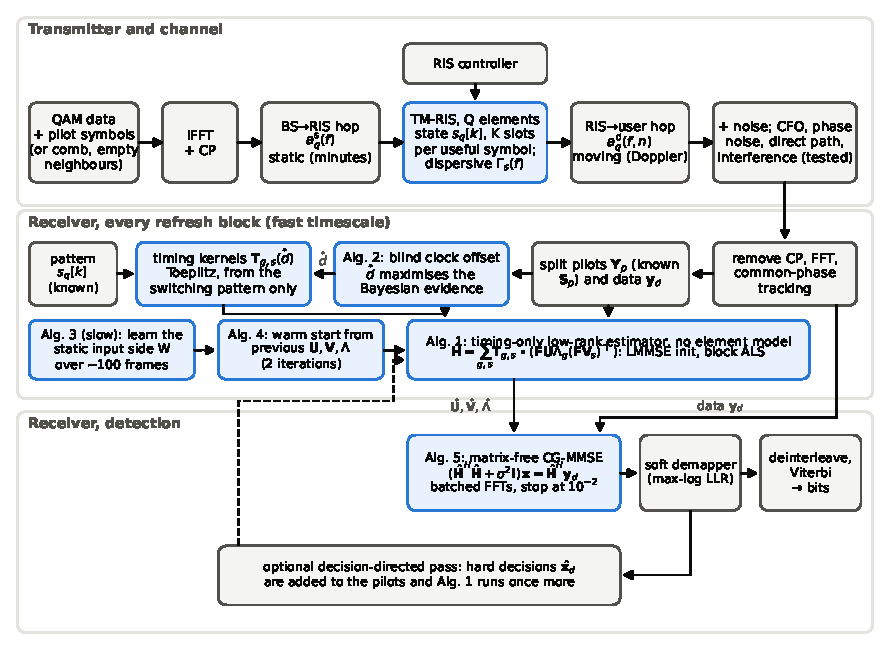
\includegraphics[width=0.95\textwidth]{figP_pipeline.pdf}
\caption{Complete system and receiver pipeline. Shaded blocks are the proposed receiver
components; each is an algorithm of Section~\ref{sec:receiver}. The receiver uses the
switching pattern (A1) and never the element model.}
\label{fig:pipeline}
\end{figure}

\subsection{Architecture}
Fig.~\ref{fig:pipeline} shows the complete pipeline. The transmitter sends $N_p$ pilot
OFDM symbols followed by data, either as full pilot symbols or as comb pilots with empty
neighbouring resource elements (Section~\ref{sec:res-pilot} shows the two are
equivalent and that data next to pilots is not). The receiver removes the cyclic prefix,
applies the FFT and, under mobility, corrects one common phase per symbol (A7). It then
(i) builds the timing kernels $\bm T_{g,s}$ from the known pattern; (ii) estimates the RIS
clock offset $\hat d$ blindly from the pilots (Algorithm~\ref{alg:offset}) and shifts the
kernels; (iii) estimates the coupling matrix in factored form (Algorithm~\ref{alg:est}),
either from scratch or warm-started from the previous refresh block (Algorithm~\ref{alg:warm}),
optionally with the static input side learned on a slow timescale (Algorithm~\ref{alg:learn});
(iv) equalizes the data matrix-free by conjugate gradients (Algorithm~\ref{alg:cg}); and
(v) computes max-log LLRs from its own estimate for a soft-input channel decoder. One
optional decision-directed (DD) pass reuses hard decisions as additional pilots. All
blocks use the factored model~\eqref{eq:model}; the $M\times M$ matrix is never formed.

\subsection{Timing-only low-rank estimation}\label{sec:est}
\emph{Model and prior.} Each hop's response is delay-limited to $[0,\tau_{\max}]$. We
represent it with the first $L$ discrete prolate spheroidal sequences (DPSS) of the
bandwidth--delay product $M\Delta f\tau_{\max}$~\cite{slepian1978,zemen2005}: $\bm F\in\mathbb C^{M\times L}$
holds the leading eigenvectors of $R_{nm}=e^{-j\pi(n-m)\Delta f\tau_{\max}}\mathrm{sinc}((n-m)\Delta f\tau_{\max})$,
and $\bm\lambda\in\mathbb R^{L}$ their eigenvalues normalized to unit sum. The DPSS basis is
the best $L$-dimensional subspace for responses with delays uniform in $[0,\tau_{\max}]$ and
has no delay grid to fall off. The eigenvalues serve as prior variances: coefficient $l$
of any hop response has prior variance $\varsigma\lambda_l$, with the scale $\varsigma$ set by
moment matching on the pilots. This prior is what keeps the estimator stable when $L$ is
larger than the effective number of delay dimensions ($M\Delta f\tau_{\max}+1\approx3.3$ at
$M=256$, $\tau_{\max}=0.3\,\mu$s, while $L=16$).

\emph{Observation model.} Pilot symbol $p$ is $\bm s_p\in\mathbb C^M$ with received $\bm y_p$.
By Corollary~\ref{cor:fft}, $\bm H\bm s_p$ is linear in each of $\bm U$, $\bm V_s$ and $\bm\Lambda_g$
when the others are fixed, with regressors built from
$\bm G_{g,s,p}=\bm T_{g,s}(\bm s_p\odot\bm F)\in\mathbb C^{M\times L}$, computed once by FFT:
\begin{align}
\bm H\bm s_p&=\textstyle\sum_g\sum_{a=1}^{r}(\bm F\bm u_a)\odot\big[\textstyle\sum_s\bm G_{g,s,p}\bm V_s\bm\Lambda_g^{\top}\big]_{:,a}\label{eq:linU}\\
&=\textstyle\sum_g\sum_s\sum_{b=1}^{r}\big[(\bm F\bm U\bm\Lambda_g)_{:,b}\odot\bm G_{g,s,p}\big]\bm v_{s,b}\label{eq:linV}\\
&=\textstyle\sum_g\sum_{a,b}\big[(\bm F\bm u_a)\odot(\textstyle\sum_s\bm G_{g,s,p}\bm V_s)_{:,b}\big]\,[\bm\Lambda_g]_{ab},\label{eq:linL}
\end{align}
which are linear in $\bm U$, in $\bm V_s$ and in $\bm\Lambda_g$, respectively.
Stacking the $N_p$ pilots gives, for each block $\bm\theta\in\{\vect\bm U,\vect[\bm V_1;\bm V_2],\vect\{\bm\Lambda_g\}\}$,
a linear model $\bm y=\bm A_{\bm\theta}\bm\theta+\bm w$, $\bm y=\vect[\bm y_1,\dots,\bm y_{N_p}]$.
With prior $\bm\theta\sim\mathcal{CN}(\bm 0,\bm P)$, $\bm P=\diag(\bm p)$, the LMMSE update is computed in
the numerically stable form
\begin{equation}
\hat{\bm\theta}=\bm P^{1/2}\big(\bm P^{1/2}\bm A_{\bm\theta}^{\mathsf H}\bm A_{\bm\theta}\bm P^{1/2}+\sigma^2\bm I\big)^{-1}\bm P^{1/2}\bm A_{\bm\theta}^{\mathsf H}\bm y,
\label{eq:lmmse}
\end{equation}
which remains well posed when some prior variances are tiny. The $\bm\Lambda$ step is a
convex least-squares problem with a small ridge ($10^{-3}$ of the mean diagonal of
$\bm A^{\mathsf H}\bm A$).

\emph{Initialization.} Ignoring the low-rank coupling between groups, $\bm H\approx\sum_s(\sum_g\bm T_{g,s})\circ(\bm F\bm C_s\bm F^{\top})$
is linear in the two $L\times L$ delay matrices $\bm C_s$. Its LMMSE estimate with prior
$\varsigma(\bm\lambda\otimes\bm\lambda)$ is exact for identical patterns ($G=1$), and its SVD,
$[\hat{\bm C}_1\;\hat{\bm C}_2]=\bm Y\bm\Sigma\bm W^{\mathsf H}$, initializes
$\bm U=\bm Y_{:,1:r}\bm\Sigma_r^{1/2}$ and $[\bm V_1;\bm V_2]=\bm W^{*}_{:,1:r}\bm\Sigma_r^{1/2}$, $\bm\Lambda_g=\bm I$.
An earlier version kept the pooled linear estimate as a fallback whenever it fitted the pilots
better. The ablation (Section~\ref{sec:res-ablation}) showed that this rule is itself an overfitting trap: the linear
model has more freedom, fits the pilots better and predicts worse, and on TDL channels at 30\,dB it was chosen in
30--57\% of channels and increased the gap. On fresh channels (pre-registered), removing it never made the gap worse
and reduced it by up to $0.25\pm0.17$\,bit/s/Hz; Algorithm~\ref{alg:est} therefore always returns the low-rank
estimate. The alternating iterations converge within one or two iterations from the SVD initialization, while random
initializations are 3--5 times worse, so the initialization matters more than the iteration count.

\begin{algorithm}[!htbp]
\caption{Timing-only low-rank estimation}\label{alg:est}
\begin{algorithmic}[1]
\Require pilots $\bm Y,\bm S$; kernels $\{\bm T_{g,s}\}$; DPSS $\bm F,\bm\lambda$; $\sigma^2$; rank $r$; iterations $I$ (20)
\State $\bm G_{g,s,p}\gets\bm T_{g,s}(\bm s_p\odot\bm F)$ by FFT \Comment{once}
\State $[\hat{\bm C}_1,\hat{\bm C}_2]\gets$ LMMSE of the pooled linear model, prior $\varsigma(\bm\lambda\otimes\bm\lambda)$
\State $\bm U,\bm V_1,\bm V_2\gets$ rank-$r$ SVD of $[\hat{\bm C}_1\;\hat{\bm C}_2]$; $\bm\Lambda_g\gets\bm I$; prior of $\bm U,\bm V_s$ columns $\propto\bm\lambda$
\For{$i=1,\dots,I$}
  \State $\{\bm\Lambda_g\}\gets$ ridge least squares (convex) \Comment{(linear in $\bm\Lambda$)}
  \State $\bm U\gets$ LMMSE~\eqref{eq:lmmse} \Comment{$Lr$ unknowns}
  \State $[\bm V_1;\bm V_2]\gets$ LMMSE~\eqref{eq:lmmse} \Comment{$2Lr$ unknowns}
\EndFor
\State $\hat{\bm H}\gets\sum_{g,s}\bm T_{g,s}\circ((\bm F\bm U)\bm\Lambda_g(\bm F\bm V_s)^{\top})$ (kept factored)
\State \Return $\hat{\bm H}$ \Comment{no pilot-fit fallback, see text}
\end{algorithmic}
\end{algorithm}

\emph{Identifiability.} The number of complex unknowns is $3Lr+Gr^2$, against $MN_p$
observations. Table~\ref{tab:unknowns} gives the counts used in the evaluation and those
of the baselines. The nominal counts are close to or above the observations at $M=256$;
the estimator is nevertheless well determined because the DPSS prior concentrates each hop
on about $M\Delta f\tau_{\max}+1$ effective dimensions. Quantitatively, the effective number of degrees of freedom of the
linear first stage, $\mathrm{tr}$ of its LMMSE hat matrix, is only 19, 22, 24 and 27 at 20\,dB (23, 27, 30, 33 at 30\,dB)
for 1, 2, 4 and 8 pilot symbols, against 256 to 2048 observations and 512 nominal unknowns: this, not the unknown
count, is why one or two pilot symbols suffice. Under the assumed prior, the Bayesian bound on the coupling-matrix
error is $-32.4$ and $-39.4$\,dB with two pilot symbols at 20 and 30\,dB; the achieved error is 5--6\,dB higher ($-26.4$,
$-34.3$\,dB), because real channels (sparse paths, exponential profiles) do not follow the uniform-delay prior. A
learned prior could close part of this gap. At the full band the low-rank form
is essential: the linear model has $2L^2=1800$ unknowns and its accuracy degrades with
bandwidth (Section~\ref{sec:res-full}), while the low-rank model has $3Lr+r^2=784$.

\begin{table}[!htbp]\centering
\caption{Complex unknowns of each estimator and pilot observations. $L=16$ at $M=256$ (fixed in calibration); $L=\lceil M\Delta f\tau_{\max}\rceil+10=30$ at the full band ($\tau_{\max}=0.2\,\mu$s); CE-BEM uses a two-hop basis with $L_2=\lceil M\Delta f\cdot0.6\,\mu s\rceil+12=17$.}
\label{tab:unknowns}
\begin{tabular}{lcc}\toprule
Estimator & unknowns & observations ($N_p=2$)\\\midrule
Ours, $M=256$, $L=16$, $r=8$, $G=1$ & $3Lr+Gr^2=448$ & 512 \\
Ours, $M=256$, $G=16$ (all patterns distinct) & 1408 & 512 \\
Ours, linear first stage, $M=256$ & $2L^2=512$ & 512 \\
Ours, $M=3276$, $L=30$, $r=8$ & 784 & 6552 \\
Ours, linear first stage, $M=3276$ & 1800 & 6552 \\
CE-BEM $|h|\le12$ / 40 / 128 / all 255 & 425 / 1377 / 4369 / 8687 & 512 \\
Unstructured banded LS ($|h|\le16$) & $33$ per row & needs $N_p\ge33$\\\bottomrule
\end{tabular}
\end{table}

\subsection{Blind recovery of the RIS clock offset}\label{sec:timing}
By Proposition~\ref{prop:offset} an unknown offset $d$ (in slots) replaces each kernel by
$\bm D_d\bm T_{g,s}\bm D_d^{*}$. For a candidate $d$, the pooled linear first stage of
Algorithm~\ref{alg:est} is a linear Gaussian model $\bm y=\bm\Phi_d\bm c+\bm w$,
$\bm c\sim\mathcal{CN}(\bm 0,\bm P)$, $\bm P=\varsigma\diag(\bm\lambda\otimes\bm\lambda,\bm\lambda\otimes\bm\lambda)$.
Its evidence (marginal likelihood) is, up to a constant,
\begin{equation}
\log p(\bm y\,|\,d)=-\bm y^{\mathsf H}\bm C_d^{-1}\bm y-\log\det\bm C_d,\qquad
\bm C_d=\bm\Phi_d\bm P\bm\Phi_d^{\mathsf H}+\sigma^2\bm I.
\label{eq:evidence}
\end{equation}
It is evaluated in the parameter domain ($2L^2$ dimensions instead of $MN_p$) with the Cholesky factor of
\[\bm B=\sigma^{-2}\bm P^{1/2}\bm\Phi_d^{\mathsf H}\bm\Phi_d\bm P^{1/2}+\bm I=\bm R^{\mathsf H}\bm R:\]
\begin{align*}
\log\det\bm C_d&=MN_p\log\sigma^2+2\textstyle\sum_i\log R_{ii},\\
\bm y^{\mathsf H}\bm C_d^{-1}\bm y&=\sigma^{-2}\|\bm y\|^2-\sigma^{-4}\|\bm R^{-\mathsf H}\bm P^{1/2}\bm\Phi_d^{\mathsf H}\bm y\|^2
\end{align*}
(Appendix~\ref{app:evidence}). The first term rewards fit; the log-determinant penalizes
models that can fit too much. A wrong offset fits through improbable shifted responses
and loses evidence even when it fits well.

\emph{The delay reference.} The prior places each hop's delays in $[t_0,t_0+\tau_{\max}]$. After
synchronization the two hops' first arrivals add to zero up to the offset, so a window that starts after the
synchronization reference ($t_0>0$) cannot hold both hops, and a late synchronization has the same effect.
We therefore let the evidence also choose $t_0$ from a small set, jointly with $d$ (Algorithm~\ref{alg:offset}):
the evidence of different priors is directly comparable.

\begin{algorithm}[!htbp]
\caption{Blind clock-offset and delay-reference estimation by evidence}\label{alg:offset}
\begin{algorithmic}[1]
\Require pilots $\bm Y,\bm S$; nominal kernels $\{\bm T_{g,s}\}$; DPSS $\bm F,\bm\lambda$; $\sigma^2$; window starts $\mathcal T_0=\{-150,-75,0,+75\}$\,ns
\For{each $t_0\in\mathcal T_0$}
  \State $\bm F_{t_0}\gets\diag(e^{-j2\pi m\Delta f t_0})\bm F$ \Comment{delays $[t_0,t_0+\tau_{\max}]$}
  \State $\mathcal E_{t_0}(d)\gets$~\eqref{eq:evidence} with kernels $\bm D_d\bm T_{g,s}\bm D_d^{*}$ and basis $\bm F_{t_0}$
  \State $d_0\gets\arg\max\mathcal E_{t_0}(d)$ over $d\in\{-0.5,-0.475,\dots,0.5\}$ slot (41 points)
  \State $\hat d_{t_0}\gets$ golden-section maximization of $\mathcal E_{t_0}$ on $[d_0-0.025,d_0+0.025]$, 14 steps
\EndFor
\State $\hat t_0\gets\arg\max_{t_0}\mathcal E_{t_0}(\hat d_{t_0})$; \Return $(\hat d_{\hat t_0},\hat t_0)$; Algorithm~\ref{alg:est} runs with these kernels and basis
\end{algorithmic}
\end{algorithm}

\subsection{Two-timescale estimation: learning the static input side}\label{sec:twoscale}
With a fixed BS and RIS, the input-side factors $\bm W_s=\bm F\bm V_s$ (BS--RIS channel and
element dispersion) do not change between frames, while $\bm U$ (user hop) does. Learning
$\bm W_s$ once from $N_f$ past frames and estimating only $\bm U$ per frame reduces the
per-frame unknowns from $3Lr+r^2$ to $Lr$ and makes the per-frame problem linear. The
principle is known for conventional RIS~\cite{hu2019twotimescale}; two details are specific
to our model. (i) \emph{Initialization from all frames.} Each frame's first-stage estimate is
$[\hat{\bm C}_{1,f}\;\hat{\bm C}_{2,f}]=\bm U_f[\bm V_1^{\top}\;\bm V_2^{\top}]$, so stacking the
frames vertically gives a matrix whose row space is the shared input side; its top-$r$ right
singular vectors initialize $\bm V_s$. (ii) \emph{Learned prior.} The learned $\bm W_s$ is an
arbitrary invertible mixture of the true input side, so the columns of $\bm U$ are correlated.
We learn $\bm R_u=\frac{1}{N_fL}\sum_f\bm U_f^{\top}\diag(\bm\lambda)^{-1}\bm U_f^{*}$ and use the
prior $\vect\bm U\sim\mathcal{CN}(\bm 0,\bm R_u\otimes\diag(\bm\lambda))$.

\begin{algorithm}[!htbp]
\caption{Learning the static input side over $N_f$ frames (slow timescale)}\label{alg:learn}
\begin{algorithmic}[1]
\Require pilots of $N_f$ frames $\{\bm Y_f,\bm S_f\}$ sharing the BS--RIS hop; $r=Q$; iterations $I_s$ (6--8)
\State stack $[\hat{\bm C}_{1,f}\;\hat{\bm C}_{2,f}]$ of the first $N_{\rm init}$ frames; $[\bm V_1;\bm V_2]\gets$ top-$r$ right singular vectors
\For{$i=1,\dots,I_s$}
  \State $\bm U_f\gets$ LMMSE given $\bm W_s=\bm F\bm V_s$, prior $\bm R_u\otimes\diag(\bm\lambda)$, for every frame
  \State $\bm R_u\gets\frac{1}{N_fL}\sum_f\bm U_f^{\top}\diag(\bm\lambda)^{-1}\bm U_f^{*}$
  \State $[\bm V_1;\bm V_2]\gets$ LMMSE over all frames jointly (normal equations accumulated frame by frame)
\EndFor
\State \Return $\bm W_s=\bm F\bm V_s$, $\bm R_u$. Per new frame: $\bm U\gets$ LMMSE given $\bm W_s$ (one linear solve)
\end{algorithmic}
\end{algorithm}

\subsection{Warm-started updates}\label{sec:warm}
When the channel is refreshed every $N$ symbols for a moving user, consecutive estimates
are close. Algorithm~\ref{alg:warm} starts from the previous factors and runs two ALS
iterations, skipping the first stage, which dominates the cost of Algorithm~\ref{alg:est}.
A cheaper variant keeps $\bm V_s$ fixed and updates only $\bm\Lambda$ and $\bm U$; its trade-off is
quantified in Section~\ref{sec:res-cost}.

\begin{algorithm}[!htbp]
\caption{Warm-started refresh}\label{alg:warm}
\begin{algorithmic}[1]
\Require new pilots; previous $\bm U,\bm V_s,\bm\Lambda_g$; iterations $I_w$ (2); flag \emph{freezeV}
\For{$i=1,\dots,I_w$}
  \State $\{\bm\Lambda_g\}\gets$ ridge LS; $\bm U\gets$ LMMSE; \textbf{if not} \emph{freezeV}: $[\bm V_1;\bm V_2]\gets$ LMMSE
\EndFor
\end{algorithmic}
\end{algorithm}

\subsection{Matrix-free equalization}\label{sec:eq}
The MMSE estimate of the data symbol solves
$(\hat{\bm H}^{\mathsf H}\hat{\bm H}+\sigma^2\bm I)\bm x=\hat{\bm H}^{\mathsf H}\bm y_d$. We use conjugate
gradients with products through~\eqref{eq:model} (Corollary~\ref{cor:fft}), as
in~\cite{hrycak2010}. For $G=1$ the product is
$\hat{\bm H}\bm x=\sum_{a}(\bm F\bm u'_a)\odot\mathcal F^{-1}\big[\sum_s\mathcal F(\bm t_s)\odot\mathcal F((\bm F\bm v_{s,a})\odot\bm x)\big]$,
where $\bm u'_a$ are the columns of $\bm U\bm\Lambda$: the forward FFTs of all $r$ columns
(and all data symbols) are one batched call per state, the two states are summed in the
frequency domain, and one batched inverse FFT follows.

\begin{algorithm}[!htbp]
\caption{Matrix-free CG-MMSE equalization}\label{alg:cg}
\begin{algorithmic}[1]
\Require $\bm y_d$ (one or several symbols as columns); factored $\hat{\bm H}$; $\sigma^2$; tolerance $\epsilon=10^{-2}$; $i_{\max}=50$
\State $\bm b\gets\hat{\bm H}^{\mathsf H}\bm y_d$; $\bm x\gets\bm 0$; $\bm r\gets\bm b$; $\bm p\gets\bm r$
\For{$i=1,\dots,i_{\max}$}
  \State $\bm q\gets\hat{\bm H}^{\mathsf H}(\hat{\bm H}\bm p)+\sigma^2\bm p$ \Comment{two batched FFT products}
  \State $\alpha\gets\|\bm r\|^2/\bm p^{\mathsf H}\bm q$; $\bm x\gets\bm x+\alpha\bm p$; $\bm r_{\rm new}\gets\bm r-\alpha\bm q$
  \State \textbf{if} $\|\bm r_{\rm new}\|/\|\bm b\|<\epsilon$ for every column \textbf{then break}
  \State $\bm p\gets\bm r_{\rm new}+(\|\bm r_{\rm new}\|^2/\|\bm r\|^2)\bm p$; $\bm r\gets\bm r_{\rm new}$
\EndFor
\State \Return $\bm x$ (columnwise scalars in practice)
\end{algorithmic}
\end{algorithm}

\subsection{Complexity}\label{sec:complexity}
Per ALS iteration of Algorithm~\ref{alg:est}, forming and solving the normal equations of the
three blocks costs (complex multiply--adds)
\begin{equation}
C_{\rm it}=\sum_{n\in\{Lr,\,2Lr,\,Gr^2\}}\Big(MN_pn^2+\frac{n^3}{3}\Big),
\label{eq:cost}
\end{equation}
and the regressors cost $2GN_pL(N_{\rm f}\log_2N_{\rm f}+2N_{\rm f})$ once ($N_{\rm f}$ the FFT length).
The first stage adds $MN_p(2L^2)^2+(2L^2)^3/3$. One evidence evaluation in Algorithm~\ref{alg:offset}
costs about the same as the first stage, and the search uses 55 of them per window start (220 for four starts). One CG iteration costs
two products of $\mathcal O(rM\log M)$ each. Table~\ref{tab:cost} evaluates these expressions;
Section~\ref{sec:res-cost} gives measured times.

\begin{table}[!htbp]\centering
\caption{Operations (complex multiply--adds) per estimate, from~\eqref{eq:cost} with $r=8$, $N_p=2$, 20 iterations, $\tau_{\max}=0.2\,\mu$s, and of the alternatives.}
\label{tab:cost}
\begin{tabular}{lccc}\toprule
 & $M=256$ & $M=1024$ & $M=3276$ \\\midrule
Algorithm~\ref{alg:est}, $G=1$ & $5.7\cdot10^{8}$ & $4.1\cdot10^{9}$ & $3.9\cdot10^{10}$ \\
Algorithm~\ref{alg:est}, $G=16$ & $1.8\cdot10^{10}$ & $5.4\cdot10^{10}$ & $1.8\cdot10^{11}$ \\
Dense MMSE solve (one symbol block) & -- & -- & $4.7\cdot10^{10}$ \\
CG equalizer, per symbol (25 it.) & -- & -- & $4.2\cdot10^{8}$ \\
Dense $\bm H$ storage & 1\,MB & 17\,MB & 172\,MB \\\bottomrule
\end{tabular}
\end{table}

\section{Evaluation Methodology}\label{sec:method}

\subsection{Setup}
Table~\ref{tab:params} lists the default parameters. Results at the full 100\,MHz n78
carrier use $M=3276$; most comparisons use $M=256$ with the same subcarrier spacing,
which preserves the per-subcarrier coupling structure at a cost that permits 10--30
independent channels per point. Only the central half of the band is scored, so that
band-edge effects do not favour any method. The receiver never uses the ground-truth
channel or the element model, except in the explicitly labelled genie and oracle references.

\begin{table}[!htbp]\centering
\caption{Default evaluation parameters.}\label{tab:params}
\begin{tabular}{ll}\toprule
Carrier, spacing & $f_c=3.594$\,GHz (n78), $\Delta f=30$\,kHz, $T_{\rm cp}=2.34\,\mu$s \\
Subcarriers & $M=256$ (central 128 scored); full band $M=3276$ (central 1638) \\
Surface & $Q=16$ elements ($4\times4$, $\lambda/2$); up to 1024 tested \\
Switching & $K=8$ slots per $T_u$, duty $D=0.75$, identical patterns (S1) unless stated \\
Element & OpenRIS cell, two states,~\cite[Table~I]{iudice2026} \\
Channel & shared paths, 1 LoS + 5 NLoS per hop, 30\,ns rms, $K_{\rm R}=10$\,dB; 3GPP TDL-A/C/D \\
Pilots & $N_p=2$ QPSK pilot symbols unless stated \\
Estimator & DPSS, $\tau_{\max}=0.3\,\mu$s, $L=16$ ($M=256$); $\tau_{\max}=0.2\,\mu$s, $L=30$ ($M=3276$); $r=8$; 20 iterations \\
TDL setting & $\tau_{\max}=\min(T_{\rm cp},10\times$ delay spread$)$, $L=\lceil M\Delta f\tau_{\max}\rceil+10$, $r=16$ \\
Equalizer & MMSE (direct at $M=256$, CG at $M=3276$) \\
SNR & $\mathrm{SNR}=P_c/\sigma^2$, $P_c$ the mean received power per subcarrier \\\bottomrule
\end{tabular}
\end{table}

\subsection{Metrics}
\emph{Achievable rate.} For an estimate $\hat{\bm H}$, the MMSE filter
$\bm W=(\hat{\bm H}^{\mathsf H}\hat{\bm H}+\sigma^2\bm I)^{-1}\hat{\bm H}^{\mathsf H}$ is applied to the
\emph{true} channel; with $\bm G=\bm W\bm H$, subcarrier $m$ has
\begin{equation}
\mathrm{SINR}_m=\frac{|G_{mm}|^2}{\sum_{n\ne m}|G_{mn}|^2+\sigma^2\|\bm w_m\|^2},\qquad
R=\frac{1}{|\mathcal M_c|}\sum_{m\in\mathcal M_c}\log_2(1+\mathrm{SINR}_m),
\label{eq:rate}
\end{equation}
over the scored set $\mathcal M_c$. The \emph{gap} is $R(\bm H)-R(\hat{\bm H})$, with $R(\bm H)$
the rate with perfect knowledge. Where losses are quoted in dB, they are the rate gap divided
by the local slope of $R$ versus SNR (0.31 and 0.33\,bit/s/Hz per dB at 20 and 30\,dB).
Under mobility,~\eqref{eq:rate} treats $G_{mm}$ as known to the detector, which amounts to
per-subcarrier gain tracking; we therefore also report two other versions. With
\emph{common-phase tracking} the receiver corrects one complex gain
$a=\hat{\bm g}^{\mathsf H}\bm g/\hat{\bm g}^{\mathsf H}\hat{\bm g}$ per symbol, where $\bm g=\diag(\bm G)$ and
$\hat{\bm g}=\diag(\bm W\hat{\bm H})$, and the residual $|g_m-a\hat g_m|^2$ adds to the interference.
With \emph{no tracking} it trusts $\hat{\bm g}$ directly. Mobility results use common-phase
tracking as the main metric (A7).

\emph{Error rates.} Uncoded symbol error rate (SER) with QAM; coded block error rate (BLER)
with a rate-1/2, constraint-length-7 convolutional code (generators 133, 171 octal), a random
interleaver, Gray-mapped 16-QAM, max-log LLRs computed from each receiver's \emph{own} estimate,
and soft Viterbi decoding, 506 information bits per block.

\emph{Net throughput.} With pilots on the first $N_p$ of every $N$ symbols, the net rate is
$R_{\rm net}=\frac{N-N_p}{N}\cdot\frac{1}{N-N_p}\sum_{n=N_p}^{N-1}R(n)$, where $R(n)$ is the rate at
symbol $n$ of the block (the estimate ages with $n$); $N$ and $N_p$ are optimized per case.

\subsection{Baselines}
All estimators use the same pilots, noise and channels, and all model-based baselines get
the same LMMSE/DPSS prior as ours, so that differences come from the model, not the
regularization.
\begin{itemize}
\item \textbf{One-tap}: per-subcarrier least squares from the pilots and one-tap
equalization: today's OFDM receiver.
\item \textbf{Toeplitz mixing}: the ideal-element model $H_{\bar mm}=t(\bar m-m)\,c(m)$ implied by
frequency-flat switching, as assumed in~\cite{tao2025secure}, estimated with our prior.
\item \textbf{CE-BEM}~\cite{tang2007}: $\bm H=\sum_{|h|\le H_b}\bm S_h\diag(\bm F_2\bm c_h)$ with
$\bm S_h$ the shift by $h$ and a two-hop DPSS basis ($0.6\,\mu$s, $L_2=17$); $H_b=4,8,12,40,128$
and all 255 harmonics; $N_p$ up to 32.
\item \textbf{OMP}~\cite{tropp2007} over a harmonic$\times$delay dictionary, stopping at the noise level or 300 atoms.
\item \textbf{Unstructured banded LS}: every entry within $|h|\le16$ estimated independently, with 32 orthogonal pilot symbols (16 times our overhead).
\item \textbf{Model-aware LMMSE} (a variant of ours): the coupling built from the \emph{exact} or a mismatched element model, to measure the value of not needing one.
\item \textbf{Equalizers} fed the same estimate and the true channel (oracle): banded MMSE with window $\pm W$~\cite{schniter2004,rugini2005}; LSQR/CG~\cite{hrycak2010}; dense MMSE.
\item \textbf{References}: perfect channel knowledge (upper bound); genie channel without phase-noise knowledge (Section~\ref{sec:res-hw}).
\end{itemize}
Deep-learning estimators were not included: they require training data matched to the
switching pattern and element, and the question studied here is the value of model structure.

\subsection{Protocol}
Each point averages 6--30 independent channel draws (stated per experiment), with 95\%
confidence intervals. Calibration (DPSS window and regularization) was done once on a
separate seed and frozen. For each experiment added after the core results, a pass/fail
criterion was written down \emph{before} running it; failed criteria are reported as failures,
with diagnosis, and follow-up methods were given new pre-registered criteria. Appendix~\ref{app:repro}
maps every table and figure to its script and result file.

\section{Results}\label{sec:results}

\subsection{Model validation}\label{sec:res-valid}
\emph{Element model.} Our implementation of~\eqref{eq:gamma} with the published parameters
reproduces the dispersion reported in~\cite{iudice2026} (Fig.~\ref{fig:dispersion}): differential
phase $172^\circ$--$184^\circ$ across 98\,MHz (reported $180^\circ\pm6.5^\circ$), magnitude imbalance
$\pm0.57$\,dB (reported $<0.75$\,dB), per-state phase variation $46.5^\circ$/$49.2^\circ$
(reported $\approx47^\circ$/$50^\circ$), ripple 0.62/0.50\,dB (reported $\approx0.6$\,dB).

\emph{Coupling model.} For $K=2$ the coupling follows the $\mathrm{sinc}(h/2)$ envelope with even
harmonics exactly zero for an ideal element; the dispersive cell creates a DC harmonic at
$-19$ to $-27$\,dB relative to $h=1$ (Fig.~\ref{fig:harmonics}). The closed form~\eqref{eq:io}
agrees with an independent time-domain simulation (per-element filtering, sampled gating, FFT;
$Q=4$, $K=4$ random patterns, multipath on both hops) to 0.27\% median and 0.49\% maximum
relative error, the residual being the sampling of the gates.

\emph{Energy collection.} Corollary~\ref{cor:parseval} predicts the gain of joint equalization
over the one-tap receiver as $(2D-1)^{-2}$. Measured with the dispersive cell (Q=16, K=8,
30 channels, Fig.~\ref{fig:energy}): 11.6, 5.9 and 2.4\,dB at $D=0.625$, 0.75 and 0.875 against
predicted 12.0, 6.0 and 2.5\,dB. At 20\,dB with perfect knowledge, the one-tap rate is 0.10,
0.42 and 1.19\,bit/s/Hz at these duty cycles, the joint MMSE rate 6.14, 6.19 and 6.11, and the
matched-filter bound 6.45, 6.52 and 6.43. Joint MMSE recovers about 95\% of the matched-filter
bound. With random per-element shifts the matrix is worse conditioned and joint MMSE reaches
5.13 against a bound of 6.62\,bit/s/Hz at $D=0.75$.

\begin{figure}[!htbp]\centering
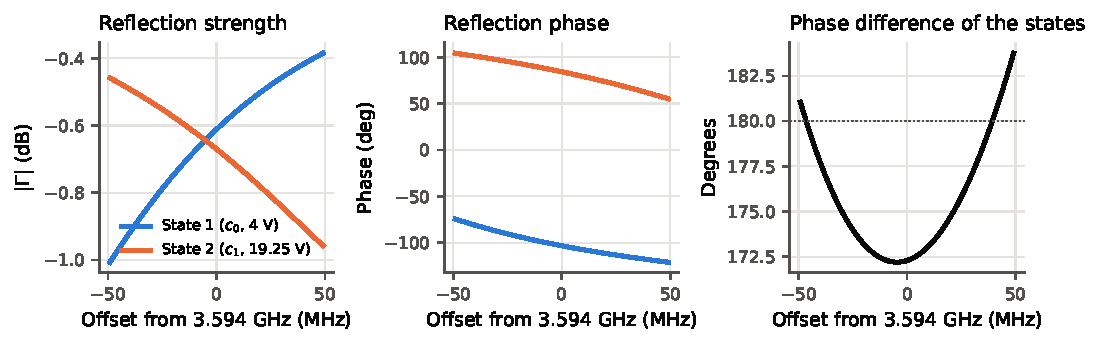
\includegraphics[width=0.9\columnwidth]{figA_element_dispersion.pdf}
\caption{Reflection magnitude, phase, and phase difference of the two states of the OpenRIS cell across the n78 carrier.}
\label{fig:dispersion}\end{figure}
\begin{figure}[!htbp]\centering
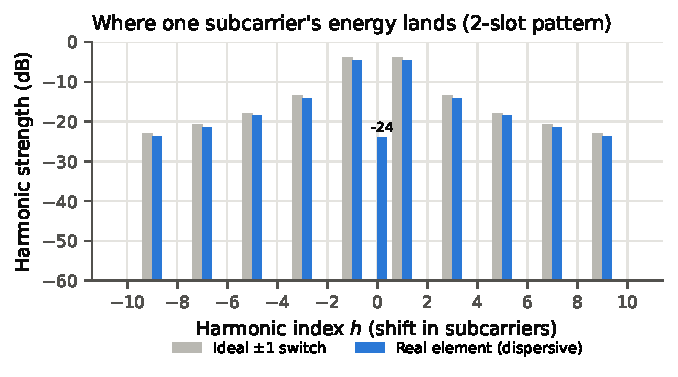
\includegraphics[width=0.75\columnwidth]{figB_harmonic_leakage.pdf}
\caption{Harmonic magnitudes for an ideal switch and the dispersive cell ($K=2$).}
\label{fig:harmonics}\end{figure}
\begin{figure}[!htbp]\centering
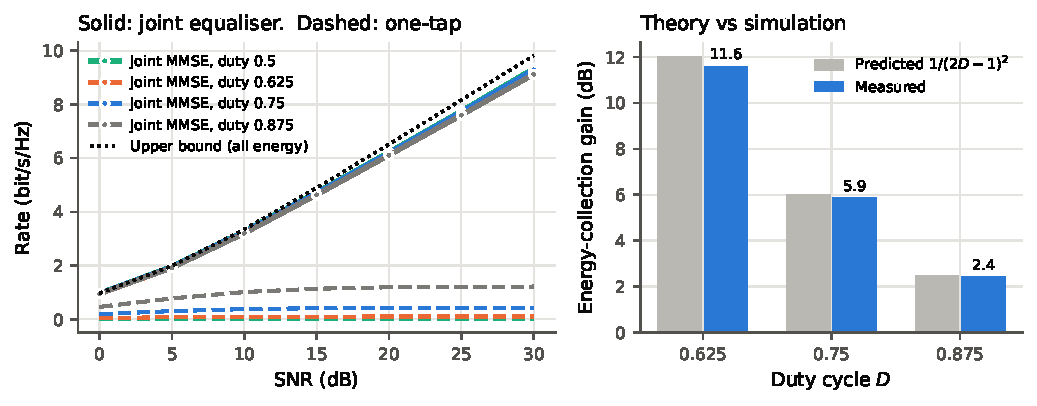
\includegraphics[width=0.9\columnwidth]{figC_energy_collection.pdf}
\caption{Left: rate of joint MMSE and one-tap versus SNR for four duty cycles. Right: predicted
$(2D-1)^{-2}$ versus measured energy-collection gain.}
\label{fig:energy}\end{figure}

\subsection{Value of not needing the element model}\label{sec:res-model}
Table~\ref{tab:model} compares receivers that differ only in what they assume about the
element (identical patterns, two pilot symbols plus two DD iterations, loss in dB against
perfect knowledge; fresh seed, 30 channels, 95\% CI on the rate loss $\le\pm0.05$\,bit/s/Hz).
A model-aware estimator with the exact model is excellent, but its accuracy collapses at high
SNR as soon as the model is wrong: a 10\,MHz resonance error costs 2.4\,dB at 30\,dB, and the
frequency-flat $\pm1$ model of earlier TM-RIS work costs 6.6\,dB. The timing-only estimator,
which uses no element model at all, is within 0.04--0.21\,dB at every SNR
(Fig.~\ref{fig:model}). This is the practical core of Corollary~\ref{cor:nomodel}: the
receiver needs only the switching timing.

\begin{table}[!htbp]\centering
\caption{Loss (dB) against perfect channel knowledge for different element knowledge. First run / confirmation run on a fresh seed (30 channels).}\label{tab:model}
\begin{tabular}{lccc}\toprule
Receiver assumes & 10\,dB & 20\,dB & 30\,dB \\\midrule
Exact element model & 0.02 & 0.05 / 0.06 & 0.12 / 0.16 \\
Resonance off by 5\,MHz & -- & 0.53 & 2.59 \\
Resonance off by 10\,MHz & 0.06 & 0.66 / 0.47 & 3.36 / 2.44 \\
Resonance off by 20\,MHz & -- & 0.55 & 2.91 \\
Ideal $\pm1$ switch (earlier TM-RIS work) & 0.18 & 1.41 / 1.42 & 6.57 / 6.60 \\
\textbf{No model, timing only (proposed)} & \textbf{0.04} & \textbf{0.08 / 0.10} & \textbf{0.11 / 0.21} \\\bottomrule
\end{tabular}
\end{table}
\begin{figure}[!htbp]\centering
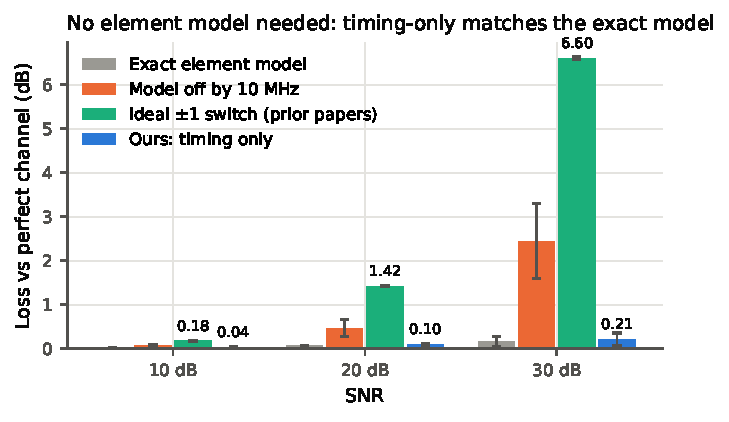
\includegraphics[width=0.75\columnwidth]{fig2_element_model_knowledge.pdf}
\caption{Loss against perfect knowledge for four assumptions about the element.}
\label{fig:model}\end{figure}

\subsection{Estimators and baselines}\label{sec:res-est}
\emph{Against the literature's estimators.} Table~\ref{tab:est} and Fig.~\ref{fig:est} compare
estimators on the same pilots and channels (20 channels, $M=256$). The one-tap receiver is
capped at its interference ratio (Corollary~\ref{cor:parseval}). The Toeplitz model of the ideal
element reaches 2.3/1.4\,bit/s/Hz: dispersion breaks its structure. CE-BEM with up to $\pm12$
harmonics reaches at most 2.3/1.4 and barely improves with pilots: by Corollary~\ref{cor:tail} it
misses 3.4\% of the coupling energy at $\pm12$. It even degrades from 20 to 30\,dB, because an
MMSE filter that trusts a wrong model hurts more when noise no longer masks the model error.
The proposed estimator is within 0.09\,bit/s/Hz (20\,dB) and 0.24\,bit/s/Hz (30\,dB) of perfect
knowledge with two pilot symbols.

\begin{table}[!htbp]\centering
\caption{Rate (bit/s/Hz) with each estimator, 20 channels, 95\% CI. $N_p$ = pilot symbols.}\label{tab:est}
\begin{tabular}{lcccc}\toprule
 & \multicolumn{2}{c}{20\,dB} & \multicolumn{2}{c}{30\,dB}\\
Estimator & $N_p=2$ & $N_p=8$ & $N_p=2$ & $N_p=8$ \\\midrule
One-tap & 0.42 & 0.42 & 0.43 & 0.43 \\
Toeplitz (ideal element) & $2.27\pm0.08$ & $2.46\pm0.10$ & $1.42\pm0.10$ & $1.52\pm0.03$ \\
CE-BEM $|h|\le4$ & $1.29\pm0.04$ & $1.33\pm0.03$ & $0.57\pm0.05$ & $0.58\pm0.02$ \\
CE-BEM $|h|\le8$ & $1.82\pm0.06$ & $1.88\pm0.04$ & $0.81\pm0.07$ & $0.99\pm0.04$ \\
CE-BEM $|h|\le12$ & $2.20\pm0.08$ & $2.32\pm0.04$ & $1.08\pm0.10$ & $1.38\pm0.06$ \\
\textbf{Proposed} & $\bm{6.52\pm0.02}$ & $\bm{6.58\pm0.02}$ & $\bm{9.68\pm0.08}$ & $\bm{9.87\pm0.02}$ \\
Perfect knowledge & 6.61 & 6.61 & 9.92 & 9.92 \\\bottomrule
\end{tabular}
\end{table}
\begin{figure}[!htbp]\centering
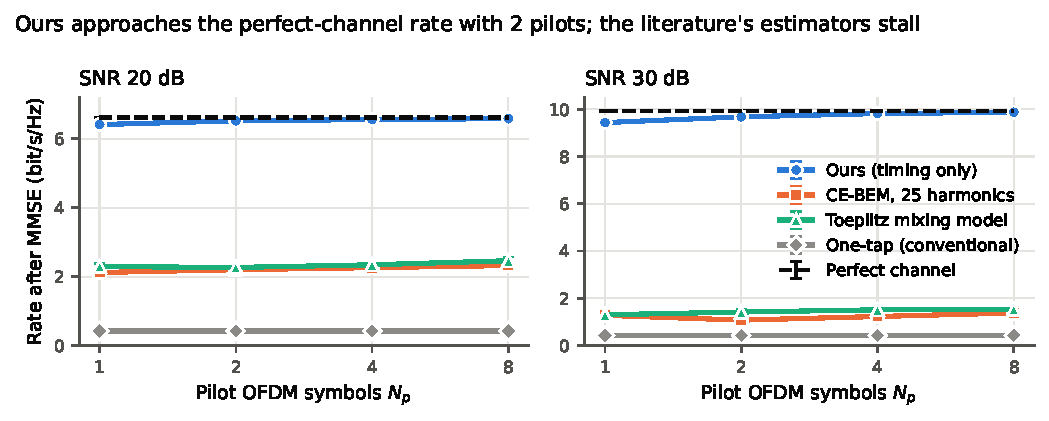
\includegraphics[width=0.85\columnwidth]{fig1_estimators_vs_pilots.pdf}
\caption{Rate versus pilot symbols at 20 and 30\,dB (20 channels, 95\% CI).}
\label{fig:est}\end{figure}

\emph{Strongest baselines.} A reviewer may object that CE-BEM failed only because it was
truncated. Table~\ref{tab:bem} gives CE-BEM with up to all 255 harmonics and up to 32 pilot
symbols (20 channels; all harmonics on 4 channels because of its 8687 unknowns). Full-harmonic
CE-BEM does approach our result, but only with 32 pilot symbols (6.18/9.37\,bit/s/Hz): the
proposed estimator with two pilot symbols (6.51/9.69) is better than full CE-BEM with 32, a
16-fold pilot saving. At equal overhead ($N_p=2$) full CE-BEM collapses to 0.13/0.08, because its
8687 unknowns cannot be determined from 512 observations. Sparse recovery (OMP) behaves like
truncated CE-BEM (2.32/1.19), and unstructured banded least squares is worst even with 32 orthogonal
pilot symbols (0.85/0.54).

\begin{table}[!htbp]\centering
\caption{Strongest baselines: rate (bit/s/Hz) at 20 / 30\,dB.}\label{tab:bem}
\begin{tabular}{lccc}\toprule
 & $N_p=2$ & $N_p=8$ & $N_p=32$ \\\midrule
CE-BEM $|h|\le12$ & 2.13 / 1.09 & 2.26 / 1.26 & 2.33 / 1.41 \\
CE-BEM $|h|\le40$ & 2.06 / 1.82 & 4.20 / 3.34 & 4.44 / 3.82 \\
CE-BEM $|h|\le128$ & 0.15 / 0.07 & 4.25 / 6.06 & 6.08 / 8.15 \\
CE-BEM all 255 harmonics & 0.13 / 0.08 & 2.97 / 4.19 & 6.18 / 9.37 \\
OMP (harmonic$\times$delay) & 2.32 / 1.19 & -- & -- \\
Unstructured banded LS & -- & -- & 0.85 / 0.54 \\
\textbf{Proposed} & \textbf{6.51 / 9.69} & -- & -- \\
Perfect knowledge & 6.59 / 9.89 & & \\\bottomrule
\end{tabular}
\end{table}

\emph{Equalizers.} Table~\ref{tab:eq} feeds the same estimate, and the true channel, to
equalizers from the high-mobility OFDM literature. Banded MMSE fails even with the true channel:
a $\pm32$ band given the true channel reaches 6.21 against 9.89\,bit/s/Hz for the dense MMSE at 30\,dB, because of the harmonic tail
(Corollary~\ref{cor:tail}). The iterative matrix-free solver matches the dense MMSE in 10
iterations, which justifies Algorithm~\ref{alg:cg}.

\begin{table}[!htbp]\centering
\caption{Equalizers on the proposed estimate (true channel in brackets), rate (bit/s/Hz).}\label{tab:eq}
\begin{tabular}{lcc}\toprule
Equalizer & 20\,dB & 30\,dB \\\midrule
One-tap & 0.42 (0.42) & 0.43 (0.43) \\
Banded MMSE $\pm4$ & 3.23 (3.24) & 3.35 (3.35) \\
Banded MMSE $\pm16$ & 4.82 (4.83) & 5.26 (5.26) \\
Banded MMSE $\pm32$ & 5.45 (5.47) & 6.20 (6.21) \\
LSQR/CG, 10 iterations & 6.51 (6.59) & 9.66 (9.83) \\
Dense MMSE & 6.51 (6.59) & 9.69 (9.89) \\\bottomrule
\end{tabular}
\end{table}
\begin{figure}[!htbp]\centering
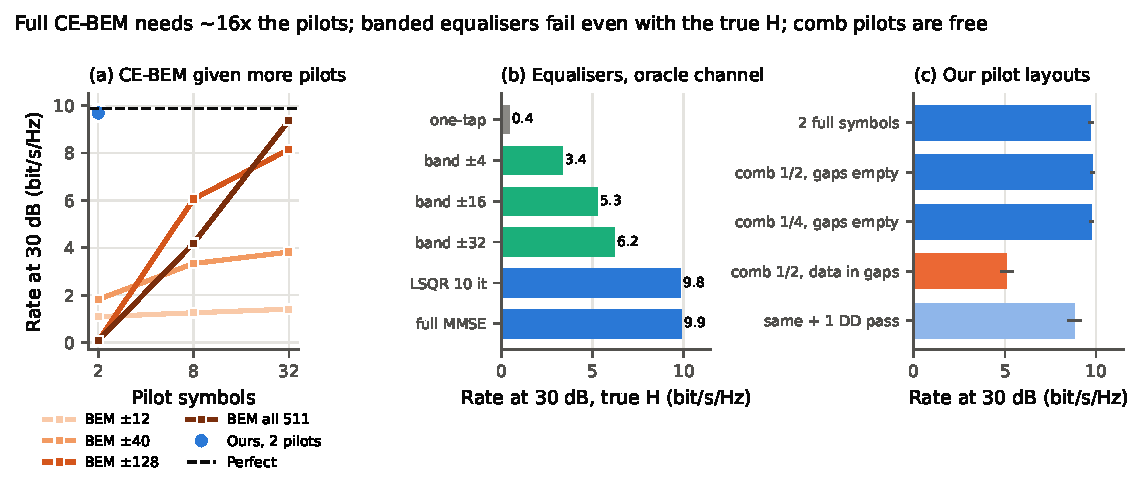
\includegraphics[width=\columnwidth]{fig16_strong_baselines.pdf}
\caption{(a) CE-BEM with more harmonics and pilots; (b) equalizers with the true channel;
(c) pilot layouts.}
\label{fig:strong}\end{figure}

\emph{Fair-case check.} Earlier TM-IRS designs choose the pattern so that the intended user sees
little coupling. Table~\ref{tab:designed} uses per-element polarities that co-phase the $h=0$
harmonic at the user. Even then the one-tap receiver saturates at its interference ratio
(3.47\,bit/s/Hz at 30\,dB for $D=0.875$, interference ratio $+10.0$\,dB), while the proposed
receiver continues to 9.37. At 10\,dB the gain is modest (+0.6\,bit/s/Hz, about 2\,dB).

\begin{table}[!htbp]\centering
\caption{User the pattern is designed for: one-tap versus proposed (estimated, $N_p=2$), bit/s/Hz at 10/20/30\,dB.}\label{tab:designed}
\begin{tabular}{lccc}\toprule
Duty, user & one-tap SIR & one-tap & proposed \\\midrule
0.875, designed & $+10.0$\,dB & 2.51 / 3.34 / 3.47 & 3.13 / 6.18 / 9.37 \\
0.75, designed & $+3.5$\,dB & 1.44 / 1.70 / 1.74 & 2.77 / 5.63 / 8.80 \\
0.625, designed & $-2.3$\,dB & 0.62 / 0.70 / 0.71 & 2.24 / 4.53 / 7.38 \\
0.75, generic & $-12.3$\,dB & 0.17 / 0.19 / 0.19 & 2.24 / 4.77 / 7.66 \\\bottomrule
\end{tabular}
\end{table}

\subsection{Full band}\label{sec:res-full}
At $M=3276$ all estimation and equalization use only the FFT operator. With the linear
first stage alone ($2L^2=1800$ unknowns) the estimate is noise-limited at $-23$ to $-29$\,dB at
28\,dB SNR (it reaches $-45$ to $-49$\,dB at 60\,dB SNR, so the model is right); the low-rank form
reaches $-39$\,dB with two pilot symbols. Table~\ref{tab:full} gives SER over 10 channels. With
pilots only, the proposed receiver's SER is 1.09$\times$ that of perfect knowledge at 20\,dB/16-QAM
and 1.54$\times$ at 28\,dB/64-QAM (an earlier 3-channel run gave 2.3$\times$); one DD pass brings
these to 1.05$\times$ and 1.14$\times$. Both numbers are reported because the DD figure alone would
overstate the pilots-only performance. A second DD pass made 64-QAM worse (SER 0.24 in an earlier
run), because decision errors feed back into the estimate; we use at most one. With per-element
cyclic shifts, the shift structure (Corollary~\ref{cor:groups}) gives an operator error of
$-34.4$\,dB at 28\,dB and SER ratios of 1.10 and 1.12 (5 channels).

\begin{table}[!htbp]\centering
\caption{Full band ($M=3276$), SER, 10 channels, 95\% CI.}\label{tab:full}
\begin{tabular}{lcc}\toprule
Receiver & 20\,dB, 16-QAM & 28\,dB, 64-QAM \\\midrule
One-tap & $0.839\pm0.003$ & $0.955\pm0.002$ \\
Perfect knowledge (CG-MMSE) & $0.031\pm0.024$ & $0.035\pm0.021$ \\
Proposed, pilots only & $0.034\pm0.025$ (1.09$\times$) & $0.054\pm0.032$ (1.54$\times$) \\
Proposed, + 1 DD pass & $0.032\pm0.024$ (1.05$\times$) & $0.040\pm0.022$ (1.14$\times$) \\
CE-BEM, pilots / + 1 DD & 0.549 / 0.563 & 0.865 / 0.865 \\\bottomrule
\end{tabular}
\end{table}
\begin{figure}[!htbp]\centering
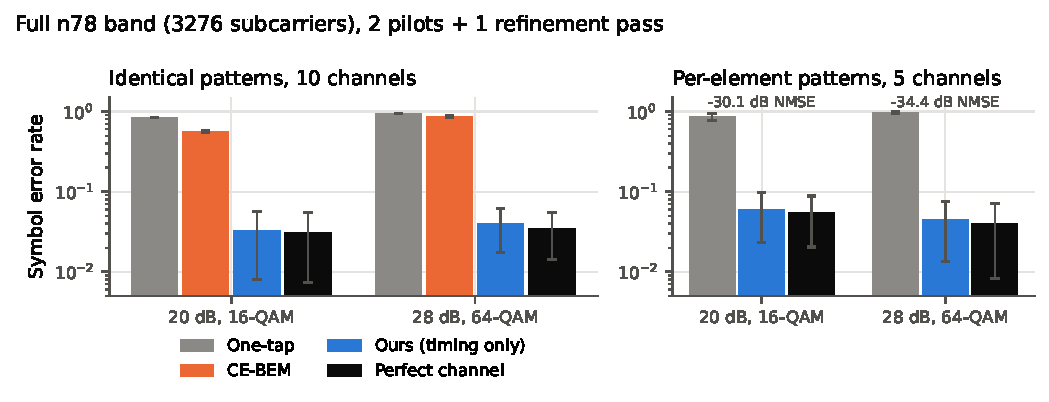
\includegraphics[width=0.85\columnwidth]{fig3_full_band.pdf}
\caption{Full-band symbol error rate for identical and per-element patterns.}
\label{fig:full}\end{figure}

\subsection{Coded performance}\label{sec:res-coded}
Fig.~\ref{fig:coded} and Table~\ref{tab:coded} give the block error rate with the convolutional
code (30 channels $\times$ 4 blocks per point). The one-tap receiver never decodes a block. CE-BEM
reaches at best 0.31 near 12--14\,dB and then degrades to 0.97 at 24\,dB, again the overconfident
wrong model. The proposed receiver reaches 0.025 at 10\,dB and no errors from 12\,dB; interpolating
in the logarithm of BLER, it crosses 10\% at 8.84\,dB against 8.46\,dB with perfect knowledge, a gap
of 0.4\,dB. Goodput saturates at the code limit of 1.98\,bit per subcarrier from 12\,dB.

\begin{table}[!htbp]\centering
\caption{Coded block error rate (rate-1/2 convolutional code, 16-QAM).}\label{tab:coded}
\begin{tabular}{lccccc}\toprule
SNR (dB) & 6 & 8 & 10 & 12 & 14--24 \\\midrule
One-tap & 1 & 1 & 1 & 1 & 1 \\
CE-BEM & 1 & 1 & 0.71 & 0.31 & 0.31--0.97 \\
Proposed & 0.93 & 0.28 & 0.025 & 0 & 0 \\
Perfect knowledge & 0.93 & 0.21 & 0.008 & 0 & 0 \\\bottomrule
\end{tabular}
\end{table}
\begin{figure}[!htbp]\centering
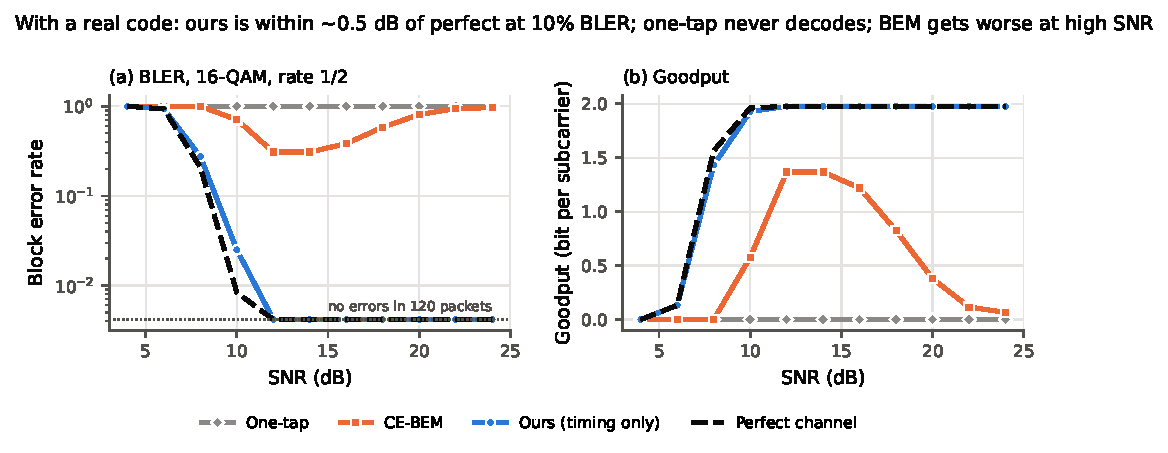
\includegraphics[width=0.9\columnwidth]{fig15_coded_bler.pdf}
\caption{Coded block error rate and goodput.}
\label{fig:coded}\end{figure}

\subsection{Sensitivity to design parameters}\label{sec:res-sweep}
Every parameter we chose was varied one at a time around the default (12 channels per point,
Fig.~\ref{fig:sweep}). The gap to perfect knowledge stays at 0.06--0.09 / 0.10--0.20\,bit/s/Hz
(20/30\,dB) for $Q=4$ to 144 elements, 0.06--0.09 / 0.11--0.16 for $K=2$ to 16 slots, and 0.05--0.13 /
0.12--0.23 for duty cycles 1/8 to 7/8. The one parameter that matters is the number $G$ of
\emph{distinct} patterns: with two pilot symbols the gap grows from 0.07 / 0.10 at $G=1$ to 0.32 / 1.03 at
$G=16$, because the unknowns grow with $Gr^2$ (Table~\ref{tab:unknowns}); four pilot symbols bring it to
0.19 / 0.38. This gives a design rule: use four pilot symbols when the surface uses many distinct
per-element patterns, as security-oriented designs do.

\begin{figure}[!htbp]\centering
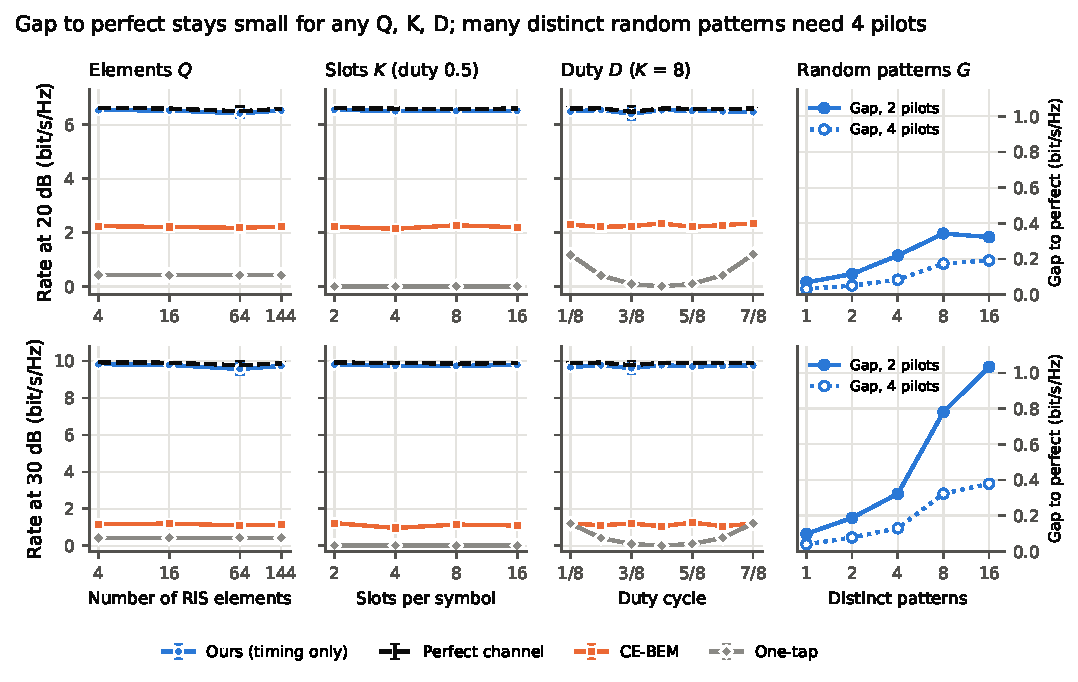
\includegraphics[width=0.85\textwidth]{fig10_parameter_sweep.pdf}
\caption{Sensitivity to the number of elements, slots, duty cycle and distinct patterns.}
\label{fig:sweep}\end{figure}

\subsection{Channel models, surface size and long delay spread}\label{sec:res-chan}
\emph{3GPP channels.} Table~\ref{tab:tdl} uses the TR~38.901 TDL models. At 30\,ns, as in the
anchor paper, two pilot symbols suffice (gap $\le0.14$ at 20\,dB). With realistic delay spreads
the default setting, designed for the six-path model, breaks: TDL channels have 14--24 taps from
different directions. Matching the delay window to the delay spread
($\tau_{\max}=\min(T_{\rm cp},10\times$DS$)$) and raising the rank to 16 fixes 100\,ns with eight
pilot symbols: gap 0.08--0.24\,bit/s/Hz at 20\,dB. The rank barely matters (8, 16 and 32 give
the same within 0.1); the number of pilots is the lever, because a longer delay window means more
unknowns (Table~\ref{tab:unknowns}). We note a correction this exposed: an earlier robustness check
to 100\,ns, made with the six-path model, was optimistic for standard channels.

\begin{table}[!htbp]\centering
\caption{Gap (bit/s/Hz) on 3GPP TDL channels at 20\,dB (30\,dB in brackets), window matched to the delay spread, ranges over ranks 8/16/32, 6 channels.}\label{tab:tdl}
\begin{tabular}{lccc}\toprule
 & $N_p=2$ & $N_p=4$ & $N_p=8$ \\\midrule
TDL-A, 100\,ns & 0.69--0.76 (2.5--2.8) & 0.21--0.32 (0.8--0.9) & \textbf{0.08--0.09} (0.24--0.27) \\
TDL-C, 100\,ns & 0.47--0.50 (1.7--1.9) & 0.17--0.24 (0.6--0.8) & \textbf{0.09--0.10} (0.18--0.26) \\
TDL-D, 100\,ns & 0.65--0.69 (2.1--2.3) & 0.31--0.37 (1.3--1.4) & \textbf{0.23--0.24} (0.85--0.95) \\
TDL-A/C/D, 300\,ns & 1.1--1.5 (3.4--4.7) & 0.6--1.1 (2.6--3.3) & 0.35--0.92 (1.4--2.3) \\\bottomrule
\end{tabular}
\end{table}

\emph{Surface size and near field.} With TDL-C at 30\,ns, $Q=64$, 256 and 1024 elements give a gap
of 0.06--0.11 / 0.17--0.25\,bit/s/Hz at 20/30\,dB with two pilot symbols: the unknowns do not grow
with $Q$ (Corollary~\ref{cor:lowrank}). With $Q=1024$ (1.3\,m aperture, Fraunhofer distance about 40\,m)
and the TDL-D line-of-sight path computed from exact element distances, a user at 3, 10 and 30\,m
sees a gap of 0.09--0.18 / 0.38--0.60 (Fig.~\ref{fig:tdl}).

\textbf{Validity warning for 300\,ns.} The cyclic-prefix condition (A2) applies to the \emph{cascade}
of both hops, and our generator gives each hop the full TDL profile. The maximum cascaded delay is
$2\times9.66$, $2\times8.65$ and $2\times12.5$ times the delay spread for TDL-A, C and D: 5.8, 5.2 and
7.5\,$\mu$s at 300\,ns, all beyond the 2.34\,$\mu$s prefix (and 2.5\,$\mu$s for TDL-D at 100\,ns, a weak
violation through taps below $-27$\,dB). The ground truth~\eqref{eq:io} assumes the prefix condition and
omits the resulting inter-symbol interference, so \emph{all 300\,ns results below are physically invalid}
and are kept only as a record; they are not claims of this paper. A valid long-delay test needs
a realistic split (e.g. a short line-of-sight BS--RIS hop) and is future work.

\emph{300\,ns (invalid, see above): learning the static side.} At 300\,ns, eight pilot symbols are not enough. With
Algorithm~\ref{alg:learn} (input side learned from 100 frames of other users or earlier positions,
$r=Q=16$), TDL-A and TDL-C reach a gap of 0.23 and 0.26\,bit/s/Hz at 20\,dB, against 0.36 and 0.46 from
one frame, and the gap at 30\,dB halves (Table~\ref{tab:300}, Fig.~\ref{fig:300}). The pre-registered
criterion (all three models $\le0.3$ at 20\,dB) nevertheless \emph{failed}, on TDL-D: it fails even when
the true static side is given (0.56), because at 300\,ns TDL-D has taps up to $12.5\times300$\,ns
$=3.8\,\mu$s, beyond the 2.34\,$\mu$s cyclic prefix (A2). Taps beyond the prefix carry about $-20$\,dB of
power, which no prefix-limited delay window can represent; a real system would switch to an extended
prefix. Two earlier versions of the learning step also failed their criteria: initializing from a single
frame gave no gain over one frame (0.37 vs 0.33 on TDL-A), and 30 frames gave 0.31. The stacked
initialization, the learned prior and 100 frames were each needed. One hundred frames is a short time
compared with the coherence of the BS--RIS hop, which is static for minutes.

\begin{table}[!htbp]\centering
\caption{300\,ns delay spread, eight pilot symbols: gap (bit/s/Hz) at 20 / 30\,dB, 6 channels.}\label{tab:300}
\begin{tabular}{lccc}\toprule
 & one frame & learned side, 100 frames & true static side \\\midrule
TDL-A & 0.36 / 1.91 & \textbf{0.23} / 0.85 & 0.12 / 0.37 \\
TDL-C & 0.46 / 1.84 & \textbf{0.26} / 0.99 & 0.12 / 0.32 \\
TDL-D & 0.85 / 2.74 & 0.64 / 2.89 & 0.56 / 1.61 \\\bottomrule
\end{tabular}
\end{table}
\begin{figure}[!htbp]\centering
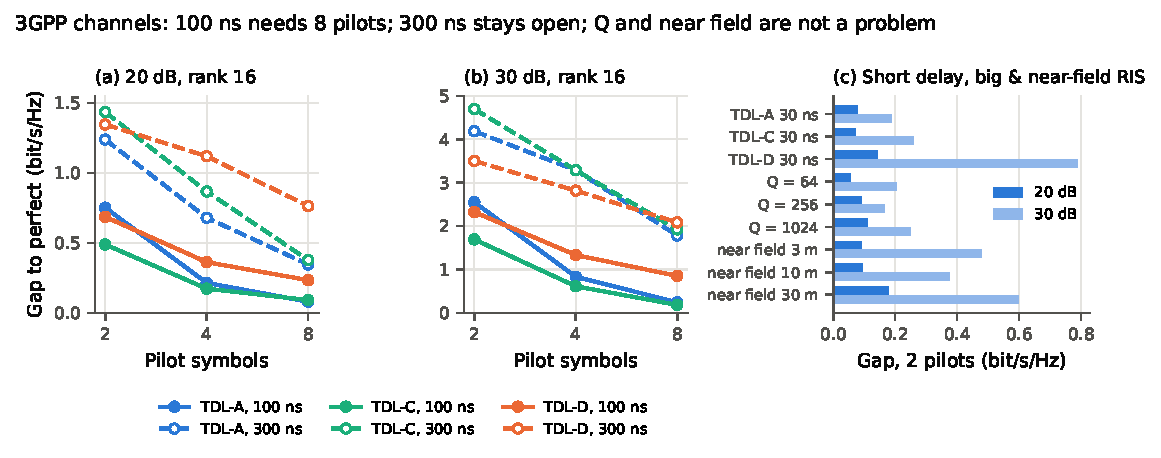
\includegraphics[width=\columnwidth]{fig14_tdl_channels.pdf}
\caption{3GPP channels: gap versus pilot symbols at 100 and 300\,ns; short delay spread, large and near-field surfaces.}
\label{fig:tdl}\end{figure}
\begin{figure}[!htbp]\centering
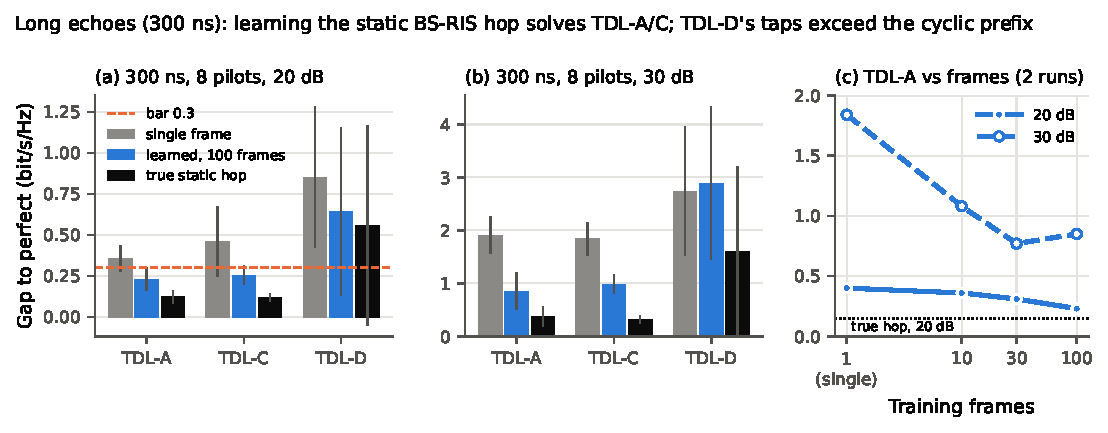
\includegraphics[width=\columnwidth]{fig21_two_timescale.pdf}
\caption{Learning the static BS--RIS side at 300\,ns delay spread.}
\label{fig:300}\end{figure}

\subsection{Timing knowledge and blind offset recovery}\label{sec:res-timing}
\emph{Sensitivity.} With the nominal timing, an unknown common offset of 0.02 slot (83\,ns) costs
4.3/11.3\,dB at 20/30\,dB, and 0.2 slot costs 15.1/25.3\,dB (Fig.~\ref{fig:timing}). The receiver must
therefore either know or estimate the offset.

\emph{Residual-based recovery.} Scanning the offset and keeping the smallest pilot residual recovers
on-grid offsets exactly (0.05, 0.20, 0.40 slot; loss within 0.03\,dB of known timing). For off-grid
offsets (uniform in $\pm0.5$ slot, grid plus golden section, 12 channels) it works at 20\,dB (0.20\,dB
vs 0.19 known) but fails at 30\,dB: rms error 0.021 slot (87\,ns), loss 4.80\,dB against 0.41\,dB
known. Refining with the full estimator and with decided data did not help (3.78\,dB). The error
grew from 20 to 30\,dB, which indicates an ambiguity rather than noise, as Proposition~\ref{prop:offset}
predicts.

\emph{A failed idea.} Since an offset is a delay, a delay window widened by a guard should absorb it
with no search. It does not (criterion failed): at 30\,dB, for offsets up to 83\,ns, the guard
window loses 2.32\,dB against 1.76\,dB without it (0.39 known); for offsets up to 208\,ns it improves
12.3 to 9.2\,dB, far from 0.28. A diagnostic showed why: the shifted responses were representable
in the plain basis already (projection error $10^{-4}$); the issue is the prior, which shrinks the
improbable shifted responses, and a wider window spreads the prior over more dimensions.

\emph{Evidence-based recovery} (Algorithm~\ref{alg:offset}) uses exactly that prior. On the same
channels and offsets as the residual search, it gives an rms error of 0.0012 slot (5\,ns) at both
20 and 30\,dB (measured against the generator's offset, which shares the delay reference of the
prior; by Proposition~\ref{prop:offset} only the rate loss is reference-free), and losses of 0.25 and 0.40\,dB against 0.25 and 0.41\,dB with the offset known
(Table~\ref{tab:timing}, Fig.~\ref{fig:blind}); the pre-registered criterion (within 1\,dB of known at
30\,dB) passed. Every one of the 12 channels at 30\,dB lies on the known-timing line, including the
three where the residual search lost more than 10\,dB.

\begin{table}[!htbp]\centering
\caption{Blind recovery of an off-grid clock offset (12 channels, $N_p=2$).}\label{tab:timing}
\begin{tabular}{lcccc}\toprule
 & \multicolumn{2}{c}{rms error (slot)} & \multicolumn{2}{c}{loss (dB)} \\
 & 20\,dB & 30\,dB & 20\,dB & 30\,dB \\\midrule
Residual search & 0.0045 & 0.0210 & 0.57 & 4.80 \\
\textbf{Evidence search (Alg.~\ref{alg:offset})} & \textbf{0.0011} & \textbf{0.0012} & \textbf{0.25} & \textbf{0.40} \\
Offset known & -- & -- & 0.25 & 0.41 \\\bottomrule
\end{tabular}
\end{table}

\emph{Jitter.} Random jitter of individual switching edges changes the pattern's shape, not only
its delay, so it is not absorbed. It must stay below about 20\,ns rms for 20\,dB operation and 4\,ns for
30\,dB (loss at 4/8/21\,ns: 0.24/0.40/0.97\,dB at 20\,dB, 0.94/2.05/5.91\,dB at 30\,dB). Microcontroller
and FPGA clocks have jitter in the picosecond range.

\begin{figure}[!htbp]\centering
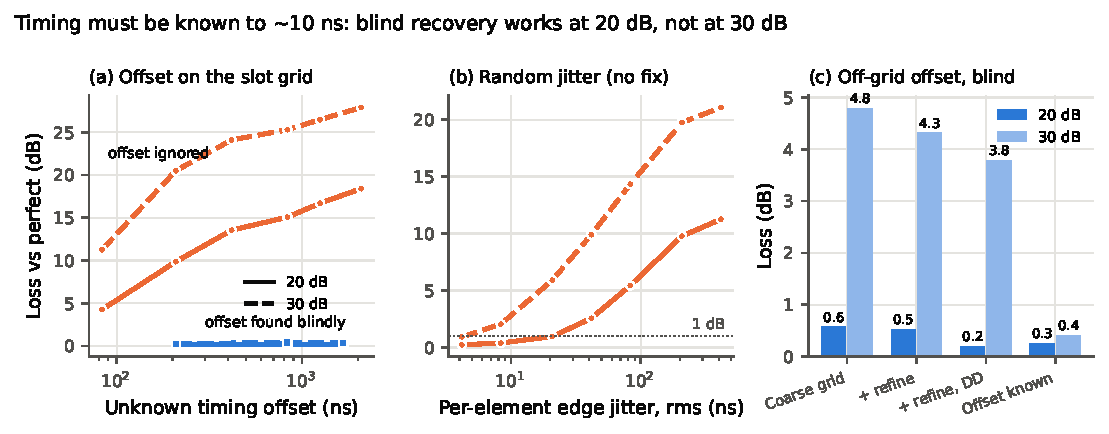
\includegraphics[width=\columnwidth]{fig12_timing.pdf}
\caption{Timing: offset sensitivity, jitter, residual-based off-grid recovery.}
\label{fig:timing}\end{figure}
\begin{figure}[!htbp]\centering
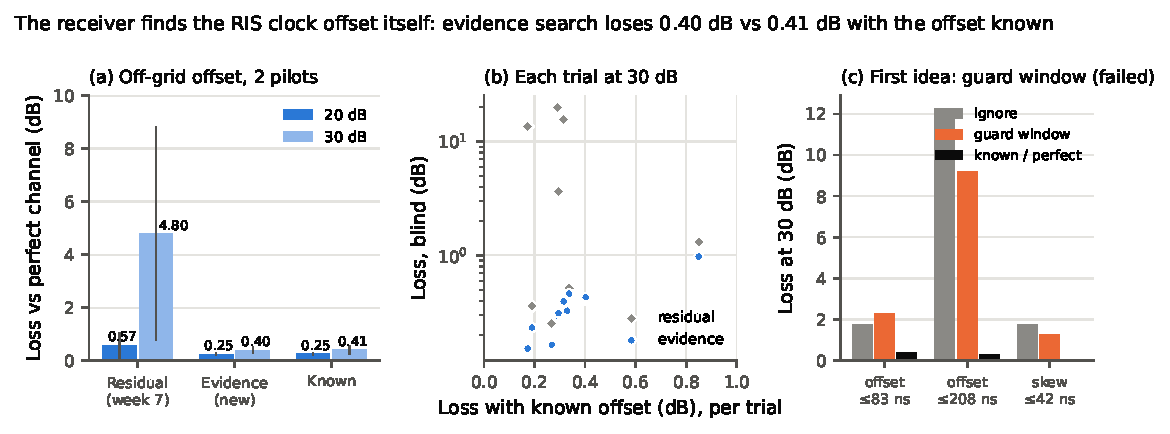
\includegraphics[width=\columnwidth]{fig20_blind_timing.pdf}
\caption{Evidence-based blind offset recovery; per-channel losses; the failed guard-window idea.}
\label{fig:blind}\end{figure}

\subsection{Hardware impairments}\label{sec:res-hw}
\emph{Element spread.} Random resonance spread of 5--20\,MHz between elements, with $\pm5\%$ loss
spread, costs 0.20--0.28 / 0.28--0.46\,dB at 20/30\,dB: the timing-only estimator never assumed
identical elements.

\emph{Switching transients.} A linear ramp between states with rise time $\rho$ (fraction of a
slot) costs up to 3.9/11.7\,dB if ignored. Building the kernels from a ramped waveform with $\rho$
calibrated once, or chosen blindly by the smallest pilot residual on a grid, brings this to
0.21--0.43 / 0.36--0.61\,dB for $\rho=0.05$--0.3; the blind estimate is within 0.03 of the true rise time.

\emph{Carrier frequency offset.} A residual CFO of 0.5/1/2/5\% of the spacing costs
0.26/0.32/0.52/1.70\,dB at 20\,dB and 0.72/1.00/2.45/7.50\,dB at 30\,dB: residual CFO must stay
below about 1\%, as standard OFDM synchronization provides.

\emph{Phase noise.} With a continuous Wiener phase over pilots and data and common-phase removal per
symbol, the fair reference is a genie that knows the channel but not the phase noise. Our receiver
adds 0.37, 0.52, 0.90 and 1.20\,dB to that reference at 20\,dB for 10, 100, 1000 and 10\,000\,Hz
linewidth (0.42, 0.99, 1.37, 1.38\,dB at 30\,dB). The pre-registered criterion (within 0.5\,dB at
$\le1$\,kHz, 20\,dB) failed at 1\,kHz and was borderline at 100\,Hz: the pilots are corrupted too.
Most of the loss, however, is the generic phase-noise ICI that any receiver suffers (the genie
itself falls from 6.63 to 4.72\,bit/s/Hz at 1\,kHz). Requirement: linewidth below about 100\,Hz at
30\,kHz spacing, or standard phase tracking (Fig.~\ref{fig:hw}).

\begin{figure}[!htbp]\centering
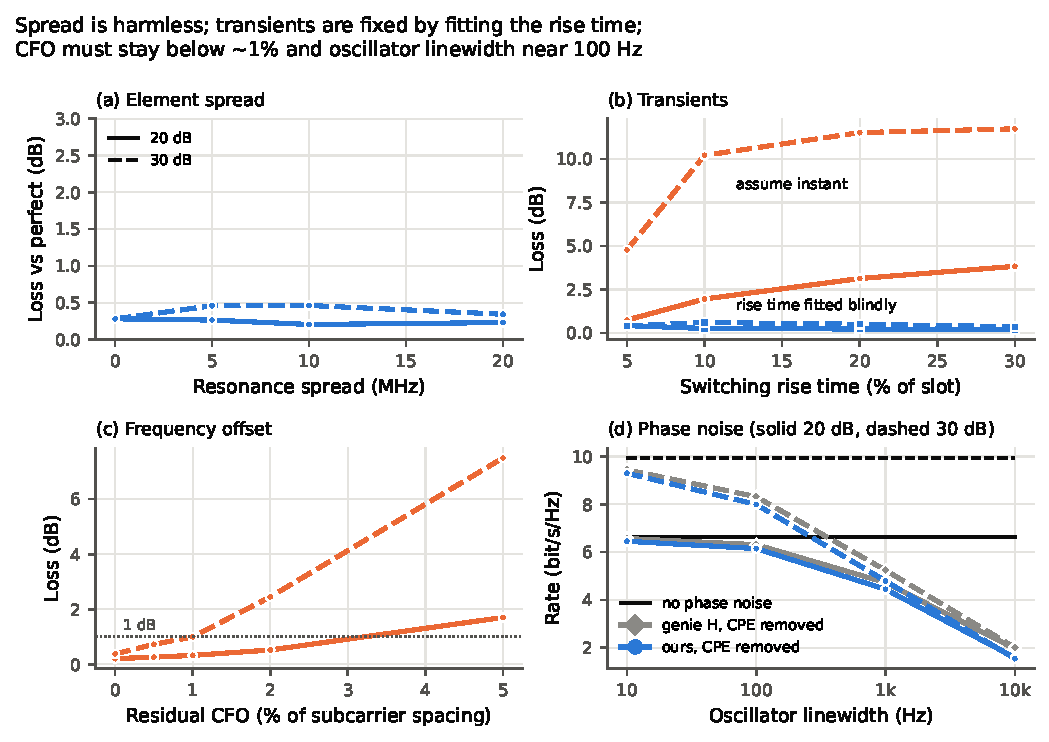
\includegraphics[width=0.85\columnwidth]{fig13_hardware.pdf}
\caption{Element spread, switching transients, CFO and phase noise.}
\label{fig:hw}\end{figure}

\subsection{Direct path, multiple panels and interference}\label{sec:res-direct}
\emph{Unblocked direct path.} A direct path at $-20$ to $+10$\,dB relative to the RIS path needs no
change to the estimator, by Corollary~\ref{cor:groups}(iii): at 0\,dB, 5.28/8.13 against 5.39/8.49
with perfect knowledge (an explicit direct-path term gives the same numbers). The one-tap receiver
improves with a strong direct path (2.9--3.1\,bit/s/Hz at $+10$\,dB) but stays far below.

\emph{Two panels.} Two TM-RIS panels with independent channels and different patterns ($G=2$): 5.54/8.67
against 5.64/8.86. A receiver that models only one panel collapses to 1.15: the receiver must know the
timing of every panel (A1).

\emph{Interference.} An unknown OFDM interferer through its own channel, treated as noise, at
SIR 20/10/0\,dB: within 0.03--0.17\,bit/s/Hz of perfect knowledge at every SIR; interference limits
both equally (Fig.~\ref{fig:direct}).

\begin{figure}[!htbp]\centering
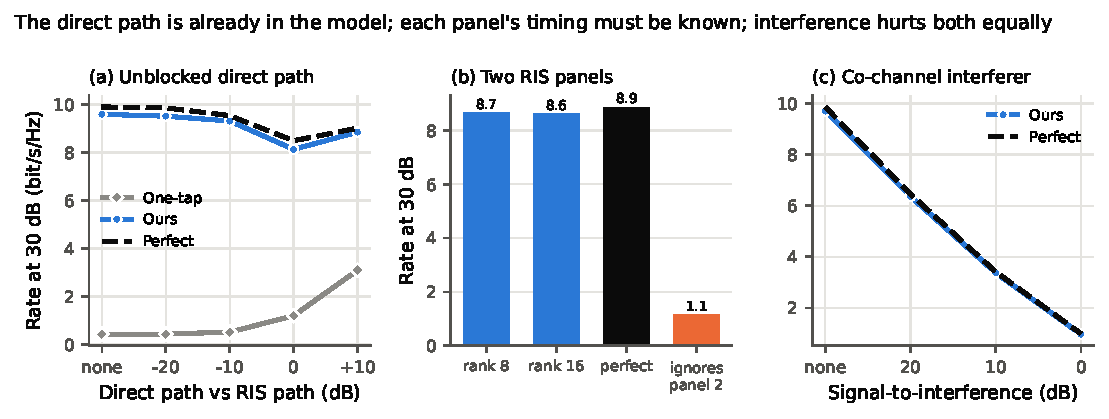
\includegraphics[width=\columnwidth]{fig17_direct_link.pdf}
\caption{Unblocked direct path, two panels, co-channel interference.}
\label{fig:direct}\end{figure}

\subsection{Pilot design}\label{sec:res-pilot}
With the same number of pilot resource elements (512) and energy: two full pilot symbols give
6.49/9.71; comb pilots on every second subcarrier over four symbols with the other resource elements
\emph{empty}, as NR DMRS allows, give 6.52/9.79; every fourth subcarrier over eight symbols, 6.51/9.77.
With \emph{data} in the gaps, the switching leaks data into the pilot bins and the rate falls to
4.79/5.10; one DD pass recovers 6.36/8.82. Design rule: comb pilots work if their neighbours are empty.

\subsection{Mobility, coherence time and pilot overhead}\label{sec:res-mob}
\emph{Coherence.} Only the RIS--user hop moves. The coherence time $T_c=0.423/f_D$ with
$f_D=vf_c/c$ is 42.4\,ms (1188 symbols) at 3\,km/h, 4.24\,ms (119 symbols) at 30\,km/h and 1.06\,ms
(30 symbols) at 120\,km/h. Doppler mixing within a symbol is $-60$, $-47$ and $-34$\,dB relative to the
signal at these speeds (0, 0.008 and 0.19\,bit/s/Hz at 30\,dB), so the main effect is the ageing of
the estimate. With one estimate reused (per-subcarrier gain metric), the gap at 20\,dB stays below 0.1\,bit/s/Hz
for more than 300 symbols at 3\,km/h, reaches 0.26 after 40 symbols at 30\,km/h (20\,dB), and 0.32 after 10
symbols at 120\,km/h (Fig.~\ref{fig:mob}).

\emph{Two failed tracking receivers.} Tracking $\bm U$ symbol by symbol from decisions, with the input
side learned, made things worse than reusing the pilot estimate (average gap over 40 symbols at 20\,dB:
0.52 against 0.28); a proper Kalman filter with propagated covariance also failed (0.46). Wrong decisions
accumulate after about ten symbols, and at 30\,dB even the first symbol after the pilots has a gap of
0.44--0.52 for every receiver, because the in-symbol Doppler mixing at 120\,km/h is not in our model.
Fast users therefore need frequent pilots, which the overhead analysis quantifies.

\emph{Net throughput.} Table~\ref{tab:overhead} and Fig.~\ref{fig:overhead} give the net rate after pilot
overhead with the refresh interval and pilot count optimized per case. After paying for its pilots,
the proposed receiver beats the best CE-BEM in every one of the 24 cases, by 1.1--4.8\,bit/s/Hz (median 2.7). On the 3GPP
channels at 20\,dB it needs 5--7\% overhead at 3\,km/h, 5--10\% at 30\,km/h and 12\% at 120\,km/h (one pilot
symbol every eight). Slow channels with long echoes prefer several pilot symbols per refresh (four, on
TDL at walking speed); fast channels prefer one pilot symbol refreshed often. The six-path model needs
less overhead at speed (1--3\% at 20\,dB) because its dominant line-of-sight path makes the Doppler mostly a common
phase, which tracking removes; the non-line-of-sight TDL numbers are the realistic ones. Without any phase
tracking, 120\,km/h requires about 25\% overhead.

\begin{table}[!htbp]\centering
\caption{Net throughput (bit/s/Hz) after pilot overhead, refresh interval and pilot count optimized per case; in brackets: pilot symbols / block length. Ours with common-phase tracking (main), its range from no tracking to a per-subcarrier genie, the best CE-BEM (best harmonic range and pilot count, same tracking), one-tap, and perfect knowledge without pilots. Shared-path: 8 channels; TDL: 4 channels per point. CE-BEM on TDL is limited to $|h|\le40$.}\label{tab:overhead}
\begin{tabular}{llcccccc}\toprule
Channel & km/h & SNR & ours & ours range & CE-BEM & one-tap & perfect\\\midrule
Shared-path, 30\,ns & 3 & 20 & 6.28 (2/120) & 5.98--6.33 & 5.14 (32/320) & 0.38 & 6.49\\
Shared-path, 30\,ns & 3 & 30 & 9.29 (2/80) & 8.43--9.47 & 6.87 (16/240) & 0.42 & 9.79\\
Shared-path, 30\,ns & 30 & 20 & 6.13 (1/40) & 5.38--6.53 & 4.83 (16/240) & 0.39 & 6.60\\
Shared-path, 30\,ns & 30 & 30 & 8.93 (1/30) & 7.21--9.40 & 6.02 (16/240) & 0.42 & 9.90\\
Shared-path, 30\,ns & 120 & 20 & 5.59 (1/160) & 3.70--6.23 & 3.43 (8/320) & 0.40 & 6.49\\
Shared-path, 30\,ns & 120 & 30 & 7.55 (1/10) & 4.40--8.56 & 2.96 (16/320) & 0.43 & 9.78\\
\midrule
TDL-A, 100\,ns & 3 & 20 & 5.05 (4/60) & 4.91--5.34 & 3.44 (16/160) & 0.33 & 5.91\\
TDL-A, 100\,ns & 3 & 30 & 6.61 (4/40) & 6.50--7.03 & 3.25 (16/120) & 0.39 & 8.94\\
TDL-A, 100\,ns & 30 & 20 & 4.70 (1/10) & 4.47--5.29 & 2.25 (8/40) & 0.34 & 6.31\\
TDL-A, 100\,ns & 30 & 30 & 5.89 (2/15) & 5.41--6.96 & 1.93 (16/60) & 0.40 & 9.54\\
TDL-A, 100\,ns & 120 & 20 & 4.26 (1/8) & 3.65--4.97 & 1.53 (16/240) & 0.34 & 6.28\\
TDL-A, 100\,ns & 120 & 30 & 5.09 (1/6) & 4.34--6.08 & 1.24 (16/240) & 0.38 & 9.51\\
\midrule
TDL-C, 100\,ns & 3 & 20 & 5.71 (4/80) & 5.55--6.02 & 3.70 (16/240) & 0.38 & 6.34\\
TDL-C, 100\,ns & 3 & 30 & 8.05 (4/60) & 7.61--8.60 & 3.33 (16/240) & 0.42 & 9.58\\
TDL-C, 100\,ns & 30 & 20 & 4.81 (1/10) & 4.69--5.20 & 2.10 (8/40) & 0.33 & 5.95\\
TDL-C, 100\,ns & 30 & 30 & 6.03 (1/8) & 5.80--6.73 & 1.73 (8/30) & 0.37 & 9.13\\
TDL-C, 100\,ns & 120 & 20 & 4.34 (1/8) & 3.65--4.95 & 1.66 (16/320) & 0.33 & 6.07\\
TDL-C, 100\,ns & 120 & 30 & 5.37 (1/6) & 4.39--6.39 & 1.39 (16/320) & 0.40 & 9.30\\
\midrule
TDL-D, 100\,ns & 3 & 20 & 5.58 (4/80) & 5.22--5.77 & 3.63 (16/160) & 0.39 & 6.25\\
TDL-D, 100\,ns & 3 & 30 & 8.06 (2/60) & 7.46--8.51 & 3.26 (16/160) & 0.40 & 9.51\\
TDL-D, 100\,ns & 30 & 20 & 5.06 (1/20) & 4.53--5.60 & 2.88 (32/320) & 0.37 & 6.49\\
TDL-D, 100\,ns & 30 & 30 & 7.06 (1/15) & 5.96--7.73 & 2.55 (16/320) & 0.42 & 9.75\\
TDL-D, 100\,ns & 120 & 20 & 3.91 (1/8) & 3.10--4.74 & 1.64 (16/160) & 0.32 & 6.13\\
TDL-D, 100\,ns & 120 & 30 & 4.94 (1/8) & 3.66--5.51 & 1.36 (16/160) & 0.34 & 9.32\\
\bottomrule
\end{tabular}
\end{table}

\begin{figure}[!htbp]\centering
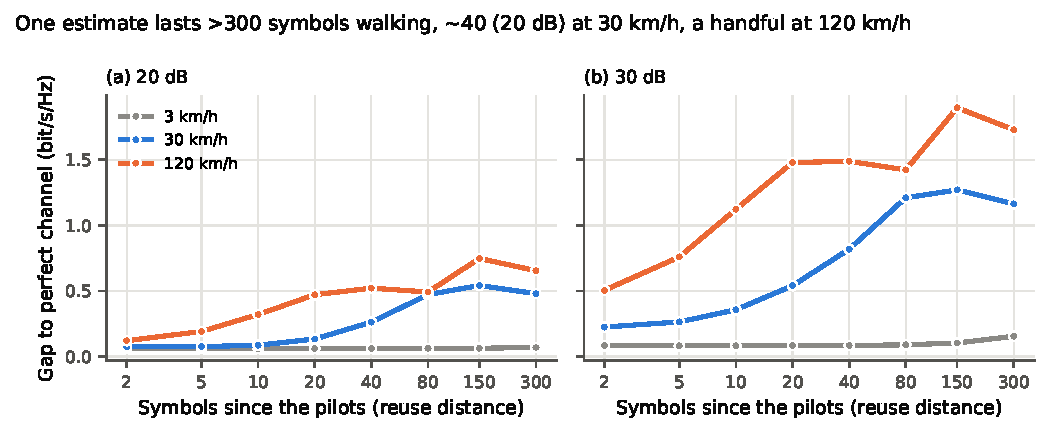
\includegraphics[width=0.8\columnwidth]{fig11_mobility.pdf}
\caption{Gap versus symbols since the pilots at 3, 30 and 120\,km/h (estimate reused).}
\label{fig:mob}\end{figure}
\begin{figure}[!htbp]\centering
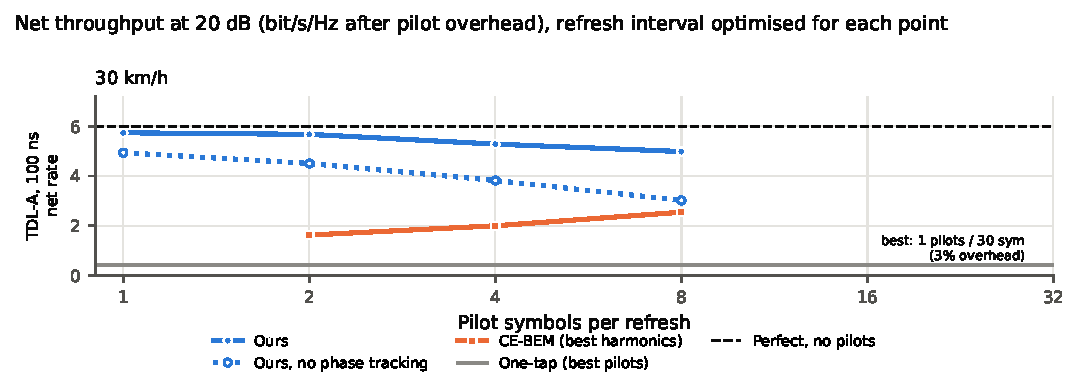
\includegraphics[width=0.85\textwidth]{fig19_pilot_overhead.pdf}
\caption{Net throughput at 20\,dB after pilot overhead versus pilot symbols per refresh.}
\label{fig:overhead}\end{figure}

\subsection{Measured cost}\label{sec:res-cost}
\emph{Updates for a moving user} ($M=256$, 30\,km/h, refresh every 20 symbols, 8 channels;
Table~\ref{tab:updates}). Warm start with two iterations needs 12$\times$ fewer operations than estimation
from scratch for 0.03\,bit/s/Hz more gap. Freezing $\bm V$ is about 100$\times$ cheaper and as good at 20\,dB,
but costs 0.23\,bit/s/Hz more at 30\,dB, because the rank-8 factorization does not split the static and
moving hops exactly; Algorithm~\ref{alg:learn} with $r=Q$ addresses this split. At the full band, a warm
update takes 1.4\,s against 12.5\,s from scratch in MATLAB (8.6$\times$), with the same SER (0.399 vs 0.398;
both estimates are 20 symbols old at 30\,km/h, which sets the absolute SER, see the caveat on tracking above).

\begin{table}[!htbp]\centering
\caption{Update variants for a moving user ($M=256$): gap at 20/30\,dB, operations, MATLAB time.}\label{tab:updates}
\begin{tabular}{lcccc}\toprule
Update & gap & operations & saving & time \\\midrule
From scratch, 20 it., $r=8$ & 0.07 / 0.17 & $1.2\cdot10^9$ & 1$\times$ & 307\,ms \\
From scratch, $r=6$ & 0.07 / 0.16 & $7.2\cdot10^8$ & 1.7$\times$ & 215\,ms \\
Warm start, 2 it. (Alg.~\ref{alg:warm}) & 0.10 / 0.20 & $1.0\cdot10^8$ & 12$\times$ & 31\,ms \\
$\bm V$ frozen, 1 it. & 0.10 / 0.40 & $1.1\cdot10^7$ & 105$\times$ & 8\,ms \\
$\bm V$ frozen, 1 pilot symbol & 0.13 / 0.49 & $6.0\cdot10^6$ & 197$\times$ & 5\,ms \\\bottomrule
\end{tabular}
\end{table}

\emph{Equalizer.} The pre-registered wall-clock comparison \emph{failed} with the element-by-element
FFT operator: at $M=3276$ CG with 25 iterations took 18.7\,s for 12 symbols against 5.6\,s for the dense
solve, with the same SER (0.065), because many small FFT calls are slow in MATLAB. With the batched
operator of Algorithm~\ref{alg:cg} and the stopping rule (a new pre-registered criterion), CG took
1.12\,s (5 iterations) against 2.95\,s dense at $M=3276$, 2.6$\times$ faster with the same SER, and
1.85\,s at $M=6552$, where the dense solve does not fit in memory (687\,MB per matrix). At $M=2048$ the
two are equal in time and the stopping rule left CG's SER 1.18$\times$ that of the dense solve, which
suggests a tighter tolerance there. The dense solve's time varied by 2$\times$ between runs with machine
load; comparisons are within a run (Fig.~\ref{fig:cost}).

\begin{figure}[!htbp]\centering
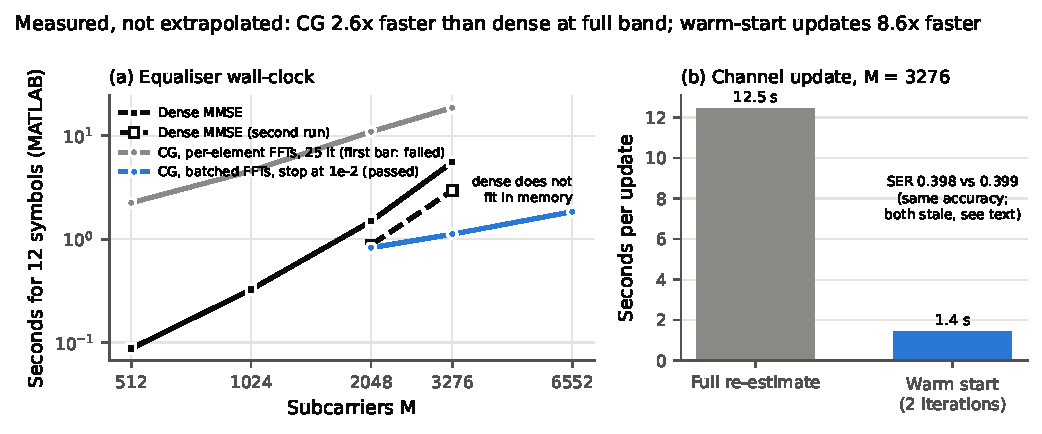
\includegraphics[width=\columnwidth]{fig22_compute_measured.pdf}
\caption{Measured equalizer time versus $M$ and full-band update time.}
\label{fig:cost}\end{figure}


\section{Trade-offs, Limitations and Scope}\label{sec:tradeoffs}

\subsection{Trade-offs}
Table~\ref{tab:tradeoffs} collects the design trade-offs of the receiver, each quantified by an
experiment of Section~\ref{sec:results}.

\begin{table}[!htbp]\centering
\caption{Design trade-offs and their measured consequences.}\label{tab:tradeoffs}
\resizebox{\textwidth}{!}{%
\begin{tabular}{p{3.6cm}p{6.2cm}p{6.6cm}}\toprule
Choice & Gain & Cost (measured) \\\midrule
Pilot symbols per refresh, $N_p$ & Accuracy: TDL 100\,ns gap 0.7 $\to$ 0.1--0.24 for $N_p=2\to8$ & Overhead $N_p/N$; for fast users one pilot refreshed often is better (net rate, Table~\ref{tab:overhead}) \\
Refresh interval $N$ & Lower overhead & Estimate ages: 120\,km/h needs $N\approx8$ on TDL (12\%); without phase tracking $N\approx4$ (25\%) \\
Delay window $\tau_{\max}$, basis size $L$ & Covers longer echoes (TDL 100\,ns needs 1\,$\mu$s) & More unknowns $\Rightarrow$ more pilots; window beyond the CP is useless (TDL-D, 300\,ns) \\
Rank $r$ & Captures more paths & Little effect between 8 and 32 on TDL; $r=6$ instead of 8 is free and 1.7$\times$ cheaper \\
Distinct patterns $G$ (security, scrambling) & Stronger scrambling for others & Unknowns $+Gr^2$: gap 0.10 $\to$ 1.03 at 30\,dB for $G=1\to16$ with 2 pilots; 4 pilots restore 0.38 \\
Duty cycle $D$ & Away from 0.5: more energy on $h=0$, better one-tap & Our receiver is indifferent (gap 0.05--0.23 for $D=1/8..7/8$); the one-tap ceiling $(2D-1)^2/(1-(2D-1)^2)$ changes \\
Decision-directed passes & 28\,dB/64-QAM: SER ratio 1.54 $\to$ 1.14 with one pass & A second pass with 64-QAM raised SER to 0.24 (error propagation); we use at most one \\
Evidence timing search & Removes the timing requirement; no rate loss vs known timing & 55 first-stage evaluations per search, about $1.2\cdot10^{12}$ operations at $M=3276$ (computed, not yet measured); needed only when the offset changes \\
Two-timescale learning & fewer per-frame unknowns (gain shown only at 300\,ns, a CP-violating case) & Needs $\sim$100 frames sharing the BS--RIS hop; stale if the BS or RIS moves \\
Warm start & 12$\times$ fewer operations (8.6$\times$ faster at full band) & +0.03\,bit/s/Hz gap \\
Freezing $\bm V$ in updates & $\sim$100$\times$ fewer operations & +0.23\,bit/s/Hz at 30\,dB unless the input side is learned with $r=Q$ \\
CG tolerance / iterations & Linear cost in $M$; fits where dense does not & Loose tolerance ($10^{-2}$) left SER 1.18$\times$ dense at $M=2048$; iterations grow with bandwidth \\
Switching rise time & Lower emission (ACLR 36.8 $\to$ 52.7\,dB for 0 $\to$ 0.05 slot) & Shrinks our advantage over truncated estimators (CE-BEM 4.7 $\to$ 8.2 at 0.3 slot); calibrated kernels needed above $\sim$40\,ns \\
Comb pilots & Same accuracy as full pilot symbols, NR-compatible & Neighbouring resource elements must be empty (data next to pilots: 9.79 $\to$ 5.10 at 30\,dB) \\\bottomrule
\end{tabular}}
\end{table}

\subsection{Limitations and scope}
\begin{itemize}
\item \emph{Simulation.} All results are simulated with one published element model; mutual
coupling between elements is ignored, as in the anchor model. Over-the-air validation is future work.
\item \emph{Pattern knowledge.} The receiver must know every panel's switching pattern (A1); with a
wrong pattern for one of two panels the rate collapses from 5.5 to 1.2\,bit/s/Hz.
\item \emph{Delay spread beyond the prefix.} Channels whose taps exceed the cyclic prefix
(TDL-D at 300\,ns) are out of scope of any prefix-limited window; 300\,ns TDL-A/C need the static
side learned over $\sim$100 frames.
\item \emph{High speed.} At 120\,km/h a pilot symbol every $\sim$8 symbols is needed on TDL
channels (12\% overhead at 20\,dB). Two tracking receivers did not improve on this, and at 30\,dB the
in-symbol Doppler mixing, not modelled by our estimator, limits every receiver. A Doppler-aware
extension of the model is future work.
\item \emph{Mobility metric.} All mobility numbers assume common-phase tracking per symbol, as in
5G NR; without it pilots are needed about twice as often.
\item \emph{Hardware.} Switching jitter must stay below about 4\,ns at 30\,dB, residual CFO below
about 1\% of the spacing, and oscillator linewidth near 100\,Hz or tracked; transients are handled by
fitting the rise time.
\item \emph{Low SNR.} At 10\,dB the gain over the one-tap receiver for a user the pattern is designed
for is modest (+0.6\,bit/s/Hz, about 2\,dB): noise, not coupling, dominates there.
\item \emph{Motivation and secrecy.} For a single user an optimized static RIS gives more rate than a TM-RIS, also with
our receiver (Section~\ref{sec:res-motiv}); our receiver reduces the cost of time modulation, it does not make it profitable.
An eavesdropper that learns the pattern can run the same receiver (secrecy rate 0.5--2.9 instead of 1.0--3.6\,bit/s/Hz at 20\,dB).
\item \emph{Rank.} With $Q=16$ and $r=8$ (or $r=Q$ in Algorithm~\ref{alg:learn}) the low-rank property
is weak; it matters for large surfaces, where it is tested only up to $Q=1024$ with narrowband array phases.
\item \emph{Equalizer speed.} The measured CG advantage counts the dense factorization against 12
symbols; with more symbols per estimate the dense factorization is amortized, and the break-even
number of symbols has not been measured.
\item \emph{Statistics.} Some points use 4--8 channels (300\,ns, TDL overhead) and the full-band
28\,dB result 10 channels; their confidence intervals are wider than those of the 20--30-channel results.
\item \emph{Learning-based estimators} were not compared (Section~\ref{sec:method}).
\end{itemize}

\section{Conclusion}\label{sec:conclusion}
The harmonic coupling of a time-modulated RIS is not unknown interference: it is the product of a
switching timing that the network sets and the receiver knows, and a propagation-plus-dispersion
part that it does not. Grouping the harmonic expansion by switching state makes this separation
exact. Built on it, a receiver needs no element model; estimates the coupling from two to eight pilot
symbols in a low-dimensional shared delay subspace; finds the RIS clock offset by itself, once one
recognizes that the offset is an opposite delay of the two hops and uses the evidence rather than
the fit; learns the static base-station side once; updates cheaply; and equalizes without forming the
coupling matrix. Against the strongest baselines we could build, including an ideal-element estimator with our prior and robust
equalizers for all, it is ahead on every channel and pilot count, exceeds with two pilot symbols a
full-harmonic basis expansion given 32,
decodes where the conventional receiver never does, and after paying for its pilots keeps
3.8--7.4\,bit/s/Hz (held-out channels) on 3GPP channels from walking speed to 120\,km/h. The limits found, delay spreads
beyond the cyclic prefix, high-speed users at high SNR, and the need to know every panel's pattern,
point to the natural next steps: a Doppler-aware coupling model, extended-prefix operation, and
over-the-air validation with a real time-modulated surface.

\appendices
\section{Energy on the original subcarrier}\label{app:parseval}
For ideal elements $\Gamma_1=+1$, $\Gamma_2=-1$ and a common pattern, the switched response is
$\gamma(t)=\mathbb 1_1(t)-\mathbb 1_2(t)\in\{\pm1\}$ with Fourier coefficients
$b^{[h]}=t_1[h]-t_2[h]$. Then $b^{[0]}=D-(1-D)=2D-1$, and by Parseval
$\sum_h|b^{[h]}|^2=\frac1{T_u}\int_0^{T_u}|\gamma(t)|^2dt=1$. A one-tap receiver uses only $b^{[0]}$:
the useful fraction is $(2D-1)^2$ and the rest, $1-(2D-1)^2$, reaches the subcarrier from its
neighbours as interference, so $\mathrm{SIR}\le(2D-1)^2/(1-(2D-1)^2)$; at $D=0.75$,
$0.25/0.75=-4.77$\,dB, and at $D=0.875$, $0.5625/0.4375=+1.09$\,dB. Joint equalization collects
the full unit energy, a gain of $1/(2D-1)^2$: 12.0, 6.02 and 2.5\,dB at $D=0.625$, 0.75 and 0.875.
The numerical sum of~\eqref{eq:tqs} over $|h|\le20000$ gives 0.99998, confirming the normalization
used for the tail fractions of Corollary~\ref{cor:tail}.

\section{Evaluating the evidence}\label{app:evidence}
Let $\bm\Phi=\bm\Phi_d$, $n=MN_p$ and $\bm P^{1/2}$ diagonal. With
$\bm C=\sigma^2\bm I+\bm\Phi\bm P\bm\Phi^{\mathsf H}$ and $\bm B=\bm I+\sigma^{-2}\bm P^{1/2}\bm\Phi^{\mathsf H}\bm\Phi\bm P^{1/2}=\bm R^{\mathsf H}\bm R$,
the matrix determinant lemma gives $\det\bm C=\sigma^{2n}\det\bm B$, and the Woodbury identity gives
$\bm C^{-1}=\sigma^{-2}\big(\bm I-\sigma^{-2}\bm\Phi\bm P^{1/2}\bm B^{-1}\bm P^{1/2}\bm\Phi^{\mathsf H}\big)$. Hence
\begin{equation}
\log p(\bm y|d)=-\frac{\|\bm y\|^2}{\sigma^2}+\frac{\|\bm R^{-\mathsf H}\bm P^{1/2}\bm\Phi^{\mathsf H}\bm y\|^2}{\sigma^4}-2\sum_i\log R_{ii}+\text{const},
\end{equation}
which needs one Cholesky factorization of a $2L^2\times2L^2$ matrix per candidate. The scale
$\varsigma$ in $\bm P$ is set per candidate by moment matching,
$\varsigma=(\|\bm y\|^2/n-\sigma^2)/(\sum_i\|\bm\phi_i\|^2p_i/n)$, as in the estimator.

\section{Derived quantities}\label{app:derived}
\emph{Coherence time.} $f_D=vf_c/c$ with $f_c=3.594$\,GHz: 9.98, 99.8 and 399.3\,Hz at 3, 30 and
120\,km/h; $T_c=0.423/f_D$~\cite{rappaport2002}: 42.4, 4.24 and 1.06\,ms; divided by
$T_s=1/\Delta f+T_{\rm cp}=35.67\,\mu$s: 1188, 119 and 30 symbols.

\emph{Unknown counts} (Table~\ref{tab:unknowns}). $L=\lceil M\Delta f\tau_{\max}\rceil+10$:
$\lceil256\cdot30\,{\rm kHz}\cdot0.3\,\mu{\rm s}\rceil=\lceil2.30\rceil=3$ is the bandwidth--delay
product, and $L=16$ was fixed in calibration; at the full band $\lceil3276\cdot30\,{\rm kHz}\cdot0.2\,\mu{\rm s}\rceil+10=\lceil19.66\rceil+10=30$.
Ours: $3Lr+Gr^2=3\cdot16\cdot8+64=448$ ($G=1$), $384+16\cdot64=1408$ ($G=16$), $3\cdot30\cdot8+64=784$
(full band). CE-BEM: $(2H_b+1)L_2$ with $L_2=\lceil256\cdot30\,{\rm kHz}\cdot0.6\,\mu{\rm s}\rceil+12=17$:
425, 1377, 4369 and 8687 for $H_b=12$, 40, 128 and 255.

\emph{Operation counts} (Table~\ref{tab:cost}) evaluate~\eqref{eq:cost} with $N_p=2$, $r=8$, 20
iterations and FFT length $N_{\rm f}=2^{\lceil\log_2 4M\rceil}$. Dense storage is $16M^2$ bytes
(complex double): 172\,MB at $M=3276$ and 687\,MB at $M=6552$.

\emph{Losses in dB} are rate gaps divided by the local slope of the perfect-knowledge rate,
0.31\,bit/s/Hz per dB at 20\,dB and 0.33 at 30\,dB, measured on the same channels.

\emph{Coded crossing.} Interpolating $\log_{10}$BLER linearly in SNR between 8 and 10\,dB:
proposed $8+2\cdot\frac{\log_{10}0.1-\log_{10}0.275}{\log_{10}0.025-\log_{10}0.275}=8.84$\,dB; perfect
knowledge $8+2\cdot\frac{\log_{10}0.1-\log_{10}0.208}{\log_{10}0.0083-\log_{10}0.208}=8.46$\,dB.

\section{Reproducibility}\label{app:repro}
All code is base MATLAB (R2026a); figures are drawn by one Python script from the saved results.
Table~\ref{tab:repro} maps every result to its script. Pre-registered criteria are recorded with
dates in the project log before the corresponding runs.

\begin{table}[h]\centering
\caption{Results and the scripts that produced them (\texttt{tm\_ris\_ofdm/matlab/}; results in \texttt{results/<script>.json}).}\label{tab:repro}
\small\begin{tabular}{p{5.6cm}p{9.6cm}}\toprule
Result & Script \\\midrule
Model validation, Fig.~\ref{fig:dispersion},~\ref{fig:harmonics} & \texttt{gate1\_reproduce}, \texttt{td\_simulate} \\
Energy collection, Fig.~\ref{fig:energy} & \texttt{gate2\_equalization} \\
Element knowledge, Table~\ref{tab:model} & \texttt{week3\_mismatch}, \texttt{week3\_modelfree}, \texttt{week3\_modelfree\_confirm} \\
Estimators, Table~\ref{tab:est} & \texttt{week4\_bem\_compare} \\
Strong baselines, Tables~\ref{tab:bem},~\ref{tab:eq} & \texttt{week7\_strong\_baselines}, \texttt{week6\_baselines\_pilots} \\
Designed user, Table~\ref{tab:designed} & \texttt{week3\_designed\_user} \\
Full band, Table~\ref{tab:full} & \texttt{week4\_fullband\_trials}, \texttt{week4\_fullband\_s2\_shift} \\
Coded, Table~\ref{tab:coded} & \texttt{week6\_coded} \\
Sensitivity, Fig.~\ref{fig:sweep} & \texttt{week5\_param\_sweep} \\
3GPP, near field, Table~\ref{tab:tdl} & \texttt{week6\_channels}, \texttt{week6\_channels\_fix} \\
300\,ns, Table~\ref{tab:300} & \texttt{week8\_twoscale\_300ns(\_b,\_c)} \\
Timing, Table~\ref{tab:timing2} & \texttt{week6\_timing(\_offgrid)}, \texttt{week7\_timing\_refine}, \texttt{week8\_timing\_guard}, \texttt{week8\_timing\_evidence}, \texttt{week9\_timing\_physics}, \texttt{week9\_timing\_landscape}, \texttt{week9\_prior\_sensitivity}, \texttt{week9\_sync\_window}, \texttt{week9\_resid\_vs\_evidence} \\
Model validity, Table~\ref{tab:mismatch} & \texttt{week9\_td\_truth}, \texttt{week9\_mismatch} \\
Hardware & \texttt{week6\_hardware(\_fix)}, \texttt{week6\_phasenoise} \\
Direct path, panels, interference & \texttt{week6\_directlink} \\
Mobility, overhead, Table~\ref{tab:overhead} & \texttt{week5\_mobility}, \texttt{week8\_tracking\_120(b)}, \texttt{week8\_pilot\_overhead} \\
Cost, Table~\ref{tab:updates}, Fig.~\ref{fig:cost} & \texttt{week7\_complexity\_fix}, \texttt{week8\_fullband\_warm}, \texttt{week8\_eq\_walltime(2,3)} \\\bottomrule
\end{tabular}
\end{table}

\begin{thebibliography}{99}
\bibitem{iudice2026} I. Iudice, D. Darsena, G. Gelli, and V. Galdi, ``Physically consistent modeling of dispersive time-modulated reconfigurable intelligent surfaces for wideband OFDM,'' arXiv:2609.18360, Sep. 2026.
\bibitem{basar2019} E. Basar, M. Di Renzo, J. de Rosny, M. Debbah, M.-S. Alouini, and R. Zhang, ``Wireless communications through reconfigurable intelligent surfaces,'' \emph{IEEE Access}, vol. 7, pp. 116753--116773, 2019.
\bibitem{wu2019} Q. Wu and R. Zhang, ``Intelligent reflecting surface enhanced wireless network via joint active and passive beamforming,'' \emph{IEEE Trans. Wireless Commun.}, vol. 18, no. 11, pp. 5394--5409, Nov. 2019.
\bibitem{zhang2018} L. Zhang \emph{et al.}, ``Space-time-coding digital metasurfaces,'' \emph{Nat. Commun.}, vol. 9, art. 4334, 2018.
\bibitem{xu2023tmirs} \TODO{first author initials} Xu and A. P. Petropulu, ``Time-modulated intelligent reflecting surface for waveform security,'' arXiv:2310.13210, 2023 (ICASSP 2024). \TODO{check}
\bibitem{tao2025gflownet} \TODO{initials} Tao and A. P. Petropulu, ``Secure time-modulated IRS via GFlowNets,'' arXiv:2506.14992, 2025. \TODO{check exact title}
\bibitem{tao2025isac} \TODO{initials} Tao, A. P. Petropulu, and H. V. Poor, ``Time-modulated IRS for integrated sensing and secure communication,'' arXiv:2509.05565, 2025. \TODO{check exact title}
\bibitem{tao2025secure} \TODO{initials} Tao, \TODO{initials} Xu, and A. P. Petropulu, ``How secure is TMA-enabled OFDM directional modulation?,'' arXiv:2310.08551, \emph{IEEE Trans. Wireless Commun.}, 2025. \TODO{check}
\bibitem{wang2026generative} K. Wang, S. Xiang, and A. Petropulu, ``Generative control of time-modulated intelligent reflecting surfaces for scalable directional modulation,'' arXiv:2610.12773, Oct. 2026.
\bibitem{verde2023} \TODO{initials} Verde, D. Darsena, and V. Galdi, ``Rapidly time-varying reconfigurable intelligent surfaces,'' arXiv:2304.11912, 2023. \TODO{check exact title}
\bibitem{tang2007} Z. Tang, R. C. Cannizzaro, G. Leus, and P. Banelli, ``Pilot-assisted time-varying channel estimation for OFDM systems,'' \emph{IEEE Trans. Signal Process.}, vol. 55, no. 5, pp. 2226--2238, May 2007.
\bibitem{zemen2005} T. Zemen and C. F. Mecklenbr\"auker, ``Time-variant channel estimation using discrete prolate spheroidal sequences,'' \emph{IEEE Trans. Signal Process.}, vol. 53, no. 9, pp. 3597--3607, Sep. 2005.
\bibitem{slepian1978} D. Slepian, ``Prolate spheroidal wave functions, Fourier analysis, and uncertainty---V: The discrete case,'' \emph{Bell Syst. Tech. J.}, vol. 57, no. 5, pp. 1371--1430, 1978.
\bibitem{tropp2007} J. A. Tropp and A. C. Gilbert, ``Signal recovery from random measurements via orthogonal matching pursuit,'' \emph{IEEE Trans. Inf. Theory}, vol. 53, no. 12, pp. 4655--4666, Dec. 2007.
\bibitem{schniter2004} P. Schniter, ``Low-complexity equalization of OFDM in doubly selective channels,'' \emph{IEEE Trans. Signal Process.}, vol. 52, no. 4, pp. 1002--1011, Apr. 2004.
\bibitem{rugini2005} L. Rugini, P. Banelli, and G. Leus, ``Simple equalization of time-varying channels for OFDM,'' \emph{IEEE Commun. Lett.}, vol. 9, no. 7, pp. 619--621, Jul. 2005.
\bibitem{hrycak2010} T. Hrycak, S. Das, G. Matz, and H. G. Feichtinger, ``Low complexity equalization for doubly selective channels modeled by a basis expansion,'' \emph{IEEE Trans. Signal Process.}, vol. 58, no. 11, pp. 5706--5719, Nov. 2010.
\bibitem{zheng2020ofdm} B. Zheng and R. Zhang, ``Intelligent reflecting surface-enhanced OFDM: Channel estimation and reflection optimization,'' \emph{IEEE Wireless Commun. Lett.}, vol. 9, no. 4, pp. 518--522, Apr. 2020.
\bibitem{wang2020compressed} P. Wang, J. Fang, H. Duan, and H. Li, ``Compressed channel estimation for intelligent reflecting surface-assisted millimeter wave systems,'' \emph{IEEE Signal Process. Lett.}, vol. 27, pp. 905--909, 2020.
\bibitem{hu2019twotimescale} C. Hu, L. Dai \emph{et al.}, ``Two-timescale channel estimation for reconfigurable intelligent surface aided wireless communications,'' arXiv:1912.07990, 2019. \TODO{full author list and journal version}
\bibitem{zhao2022multiris} \TODO{authors}, ``Cooperative reflection and synchronization design for distributed multiple-RIS communications,'' arXiv:2205.02426, 2022.
\bibitem{chen2024sr} H. Chen, R. Long, Y.-C. Liang, and R. Schober, ``Blind timing estimation and signal detection for RIS-assisted symbiotic radio with imperfect symbol synchronization,'' in \emph{Proc. IEEE ICC}, 2024, pp. 4155--4160.
\bibitem{access2019bayes} \TODO{authors and exact title}, Bayesian model selection for OFDM channel estimation under residual timing offsets, \emph{IEEE Access}, 2019 (University of Glasgow eprint 188514).
\bibitem{hku2010} \TODO{authors and exact title}, multi-model averaging over timing offset and channel length for CFO estimation, \emph{IEEE Trans. Wireless Commun.} (letter), 2010 (HKU repository 10722/124742).
\bibitem{liu2021tscatter} X. Liu \emph{et al.}, ``Verification and redesign of OFDM backscatter,'' in \emph{Proc. USENIX NSDI}, 2021. \TODO{check author list}
\bibitem{bsici2024} \TODO{authors}, ``Inter-carrier interference reduction technique for backscattered OFDM,'' 2024. \TODO{venue}
\bibitem{sr2024free} \TODO{authors}, ``Interference-free backscatter communications for OFDM-based symbiotic radio,'' arXiv:2408.09192, 2024.
\bibitem{stcisac2025} \TODO{authors}, ``Integrated sensing and communication based on space-time-coding metasurfaces,'' \emph{Nat. Commun.}, 2025.
\bibitem{stcdiff2025} \TODO{authors}, ``Space-time coded differential modulation for reconfigurable intelligent surfaces,'' arXiv:2508.10244, 2025.
\bibitem{plc_lptv} \TODO{authors}, ``Cyclic short-time varying channel estimation in OFDM power-line communication,'' \TODO{venue, year}.
\bibitem{mackay1992} D. J. C. MacKay, ``Bayesian interpolation,'' \emph{Neural Comput.}, vol. 4, no. 3, pp. 415--447, 1992.
\bibitem{rappaport2002} T. S. Rappaport, \emph{Wireless Communications: Principles and Practice}, 2nd ed. Upper Saddle River, NJ, USA: Prentice Hall, 2002.
\bibitem{tr38901} 3GPP, ``Study on channel model for frequencies from 0.5 to 100 GHz,'' TR 38.901.
\bibitem{ts38104} 3GPP, ``NR; Base Station (BS) radio transmission and reception,'' TS 38.104.
\bibitem{ts38211} 3GPP, ``NR; Physical channels and modulation,'' TS 38.211.
\end{thebibliography}

\end{document}
